\documentclass[
% papersize
a4paper,
%fond size
%12pt,
11pt,
%page print style
twoside,
%oneside,
openright]{book}

%for PSTRicks
\usepackage[pdf]{pstricks}
\usepackage[off]{auto-pst-pdf}

%graphics included tikz & pfg
\usepackage{graphicx}
\usepackage{epsfig,epic,eepic}
\usepackage{psfrag}
\usepackage[USenglish,german]{babel}
\usepackage{color,pstricks}
\usepackage{tikz}
\usepackage{ctable}
\usepackage[utf8]{inputenc}
\usepackage{wrapfig}

\usepackage[titletoc]{appendix}

% Fonts
%\usepackage{lmodern}
%from Ruben \usepackage[T1]{fontenc}
\usepackage{times}
%\usepackage[scaled]{helvet}
%\usepackage[sc]{mathpazo} % math fonts for Palatino, see
                          % http://www.tug.dk/FontCatalogue/palatino/
%\usepackage{palatino}

% Math packages
\usepackage{amsmath,amssymb,amsfonts,amsthm}
\usepackage{url}
\usepackage[ruled,noline]{algorithm2e}
% More compact lists
\usepackage{paralist}
% Fullpage
\usepackage[in,headings]{fullpage}
% But then adapt spacing
\usepackage{setspace}
\setstretch{1.3}

%for nice tables
\usepackage{multirow}
%\usepackage{booktabs}

% For SI Unit conform output
\usepackage[binary-units = true]{siunitx}

%for nice item lists
\usepackage{paralist}

%usepackage comment for block comments
\usepackage{comment}

%nice symbols to draw arrow (yes) and -(no)
\usepackage{pifont}
\newcommand{\yes}{\checkmark}
\newcommand{\no}{\textendash}

%sub-picture numbering
\usepackage{caption}
\usepackage{subcaption}
%\usepackage{subfigure}

\usepackage[right]{eurosym}


%annotate TODO stuff
\usepackage[colorinlistoftodos, textwidth=4cm, shadow]{todonotes}
\usepackage{lscape}
\usepackage{epstopdf}
%pseudocode package
\usepackage{pseudocode}

%for pdf includes
\usepackage[final]{pdfpages}

% allow captions for listings
\usepackage{newfloat}
\DeclareFloatingEnvironment[placement={!ht},name=List]{mylist}

%to insert some clickable links
\usepackage{hyperref}
\definecolor{darkblue}{rgb}{0,0,.5}
\definecolor{black}{rgb}{0,0,0}
\hypersetup{colorlinks=true, breaklinks=true, citecolor=black, linkcolor=black, menucolor=black, urlcolor=black}

% Allow code blocks
\usepackage{listings}

% Add syntax highlighting for json
\definecolor{eclipseStrings}{RGB}{42,0.0,255}
\definecolor{eclipseKeywords}{RGB}{127,0,85}
\definecolor{bground}{HTML}{f2f2f2}
\colorlet{numb}{magenta!60!black}

\lstdefinelanguage{json}{
    basicstyle=\normalfont\ttfamily,
    commentstyle=\color{eclipseStrings}, % style of comment
    stringstyle=\color{eclipseKeywords}, % style of strings
    numbers=left,
    numberstyle=\scriptsize,
    stepnumber=1,
    numbersep=8pt,
    showstringspaces=false,
    breaklines=true,
    frame=lines,
    backgroundcolor=\color{bground}, %only if you like
    string=[s]{"}{"},
    comment=[l]{:\ "},
    morecomment=[l]{:"},
    literate=
        *{0}{{{\color{numb}0}}}{1}
         {1}{{{\color{numb}1}}}{1}
         {2}{{{\color{numb}2}}}{1}
         {3}{{{\color{numb}3}}}{1}
         {4}{{{\color{numb}4}}}{1}
         {5}{{{\color{numb}5}}}{1}
         {6}{{{\color{numb}6}}}{1}
         {7}{{{\color{numb}7}}}{1}
         {8}{{{\color{numb}8}}}{1}
         {9}{{{\color{numb}9}}}{1}
}

% \setlength{\oddsidemargin}{-0.3cm}
% \setlength{\evensidemargin}{-0.3cm}
% \setlength{\textwidth}{16cm}
% \setlength{\topmargin}{-0.8cm}
% \setlength{\textheight}{23.0cm}

% use some common definitions
\newcommand{\pref}[1]{Part~\ref{#1}}
\newcommand{\cref}[1]{Chapter~\ref{#1}}
\newcommand{\sref}[1]{Section~\ref{#1}}
\newcommand{\aref}[1]{Appendix~\ref{#1}}
\newcommand{\fref}[1]{Figure~\ref{#1}}
\newcommand{\tref}[1]{Table~\ref{#1}}
\newcommand{\eref}[1]{(\ref{#1})}

% More convenient sometimes
\newcommand{\ie}{i.\@e.\@ }
\newcommand{\eg}{e.\@g.\@ }

\newcommand{\us}{\,$\mu$s\xspace}

%add empty page macro
\newcommand{\blankpage}{
\newpage
\thispagestyle{empty}
\mbox{}
\newpage
}

% Some math definitions

%\newcommand{\indic}{1\hspace{-2.5mm}{1}}
%\newcommand{\indic}{\boldsymbol{1}}
\newcommand{\indic}[1]{1_{\{#1\}}}
\newcommand{\erfc}{\mathrm{erfc}}
\newcommand{\abs}[1]{\left\lvert #1 \right\rvert}
\newcommand{\lp}[1]{\left( #1 \right)}
\newcommand{\lb}[1]{\left\lbrack #1 \right\rbrack}
\newcommand{\lc}[1]{\left\lbrace #1 \right\rbrace}
\newcommand{\erf}[1]{\mathrm{erf}\lp{#1}}
\newtheorem{definition}{Definition}
\newtheorem{lemma}{Lemma}
\newtheorem{theorem}{Theorem}

\newcommand{\calI}{\mathcal I}
\newcommand{\calN}{\mathcal N}
\newcommand{\calP}{\mathcal P}
\newcommand{\calX}{\mathcal X}
\newcommand{\calC}{\mathcal C}

% Paper specific notation
\def\su{^{(u)}}
\def\s0{^{(0)}}
%
\def\Xr{X^{(r)}}
\def\Xt{X^{(t)}}
%
\def\Ns{N_{\textrm{s}}}
\def\Na{N_{\textrm{a}}}
%
\def\tacq{t_{\textrm{acq}}}
\def\ttx{t_{\textrm{tx}}}
\def\tfail{t_{\textrm{fail}}}
\def\tdrop{t_{\textrm{drop}}}
%
\def\tprop{t_{\textrm{prop}}}
\def\tpreamble{t_{\textrm{preamble}}}
\def\tdata{t_{\textrm{DATA}}}
\def\tack{t_{\textrm{ACK}}}
\def\tsigidle{t_{\textrm{SIGIDLE}}}
\def\tmaxbackoff{t_{\textrm{max backoff}}}
\def\tsendtimer{t_{\textrm{send timer}}}
\def\tidletimer{t_{\textrm{idle timer}}}
\def\tbackoff{t_{\textrm{backoff}}}
%
\def\SD{S_{\textrm{D}}}
\def\SI{S_{\textrm{I}}}
%
\def\Pacq{p_{\textrm{acq}}}
\def\Pfail{p_{\textrm{fail}}}
\def\Pbusy{P_{\textrm{busy}}}
\def\Pmd{P_{\textrm{MD}}}
\def\Pfa{P_{\textrm{FACQ}}}
%
\def\td{t_{\textrm{D}}}
\def\ti{t_{\textrm{I}}}
\def\Np{N_{\textrm{p}}}


\newcommand{\mand} {\mathrm{\;  and \; }}
\newcommand{\mfor} {\mathrm{\;  for \;  }}
\def\Ints{\mathbb{Z}}
\def\P{\mathbb{P}}
\def\E{\mathbb{E}}
\def\be{\begin{equation}}
\def\ee{\end{equation}}
\def\ben{\[}
\def\een{\]}
\def\bearn{\begin{eqnarray*}}
\def\eearn{\end{eqnarray*}}
\def\bear{\begin{eqnarray}}
\def\eear{\end{eqnarray}}
\def\barr{\begin{array}}
\def\earr{\end{array}}
\def\bel{\be \barr{l}}% equation array adjusted left, numbered
\def\eel{\earr\ee}
\def\beln{\ben \barr{l}}% equation array adjusted left, no number
\def\eeln{\earr\een}\def\be{\begin{equation}}
\def\ee{\end{equation}}
\def\ben{\[}
\def\een{\]}
\def\bearn{\begin{eqnarray*}}
\def\eearn{\end{eqnarray*}}
\def\bear{\begin{eqnarray}}
\def\eear{\end{eqnarray}}
\def\barr{\begin{array}}
\def\earr{\end{array}}
\def\bel{\be \barr{l}}% equation array adjusted left, numbered
\def\eel{\earr\ee}
\def\beln{\ben \barr{l}}% equation array adjusted left, no number
\def\eeln{\earr\een}


% Style headings + headers and footers

% Modify header and footers
\usepackage{fancyhdr}
\pagestyle{fancy}
\fancyhf{}
\renewcommand{\chaptermark}[1]{
  \markboth{\thechapter.\ #1}{}
%  \markboth{#1}{}
}
\renewcommand{\sectionmark}[1]{
%  \markboth{\thechapter.\ #1}{}
  \markright{#1}
}

% \fancyhead[LE]{\normalfont\sffamily\thepage}
% \fancyhead[RE]{\normalfont\sffamily\leftmark}
% \fancyhead[LO]{\normalfont\sffamily\rightmark}
% \fancyhead[RO]{\normalfont\sffamily\thepage}
\fancyhead[LE]{\normalfont\thepage}
\fancyhead[RE]{\normalfont\leftmark}
\fancyhead[LO]{\normalfont\rightmark}
\fancyhead[RO]{\normalfont\thepage}

% Modify the fonts for the chapters, section, sub... and paragraphs
\usepackage{titlesec}

\titleformat{\chapter}[display]
%{\normalfont\Huge\sffamily}
{\normalfont\Huge}
{\filleft{\textbf{\LARGE{\chaptername} {\thechapter}}}}{1em}{\filleft\textbf}

\titleformat{\section}
{\normalfont\Large}
{\filright{\textbf{\thesection}}}{1em}{\filright\textbf}

\titleformat{\subsection}
{\normalfont\normalsize}
{\filright{\textbf{\thesubsection}}}{1.3em}{\filright\textbf}

\titleformat{\subsubsection}
{\normalfont\normalsize}
{}{0em}{\filright\textbf}

\titleformat{\paragraph}[runin]
{\normalfont\normalsize}
{}{0em}{\filright\textbf}

% Do it for theorems,... too
%\theoremstyle{definition}
%\newtheorem{define}{\textbf\normalfont\normalsize\sffamily{Definition}}[chapter]
%\theoremstyle{plain}
%\newtheorem{theorem}{\textbf\normalfont\normalsize\sffamily{Theorem}}[chapter]
%\newtheorem{lem}{\textbf\normalfont\normalsize\sffamily{Lemma}}[chapter]


% The larger it is, the less willing LaTeX is to split footnotes
\interfootnotelinepenalty=10000


% Removing master, slows down the compilation
\includeonly{
	title,
	abstract,
	abstract_de,
	acknowledgments,
	paper-collaborators,
	eid,
	chapter-1_introduction,
	chapter-2_related_work,
	chapter-3_software_design,
	chapter-4_measurement_tools,
	chapter-5_results,
	chapter-6_conclusion,
	appendix,
}


% BEGINN of COCUMENT
\begin{document}

\setlength{\headheight}{13.6pt}

%TITLE PAGE
\pagestyle{empty}
% Titeseite

\begin{titlepage}
  \begin{center}
	  
    %\mbox{}

    %\vspace{1cm}

	\centering
	
\includegraphics[width=15cm]{figures/Q03_HTW_Berlin_Logo_quer_pos_FARBIG_RGB.eps}\\
	\vspace{0.8em}
	\LARGE 
    \sffamily \LARGE \Huge{\textbf{Community friendly tracking of Hardware Target Distributions and Software releases}}

	\vspace{1cm}
	
	\large Master Thesis

    \vspace{1cm}

    \normalsize Informations- und Komminkationstechnik\\
    \normalsize Fachbereich I -- Ingenieurwissenschaften - Energie und Information\\
    
    \vspace{1cm}
    
    \large \textbf{Submitted By:}\\
    \Large Stefan Venz


  %  von der Fakult�t IV - Elektrotechnik und Informatik der Technischen Universit�t Berlin



    %\vspace{.1cm}
    %\normalsize der Hochschule für Technik und Wirtschaft Berlin\\
    %\vspace{.1cm}
    %\normalsize zur Erlangung des akademischen Grades\\
    %\vspace{.1cm}
    %\large \textsc{Bachelor of Engineering (B. Eng.)}\\
    %\vspace{.1cm}
    %\normalsize genemigte Bachelorarbeit\\

    \vspace{1cm}

    \large \textbf{Submitted To:}\\
        \vspace{2mm}
		\begin{tabular}{rl}
			& Prof. Dr.-Ing. Thomas Scheffler, HTW Berlin\\
			& Prof. Dr.-Ing. Thomas Hühn, Hochschule Nordhausen\\
			%ToDo: is our adress needed here ?
		\end{tabular}\\

    \vspace{2cm}

    \large Berlin, April 2021\\

  \end{center}
\end{titlepage}


\selectlanguage{USenglish}

%ABSTRACT_EN
\frontmatter \pagestyle{plain}
\setcounter{page}{1}
\addcontentsline{toc}{chapter}{Abstract}
\chapter*{Abstract}
\label{chap:abstract}

%
Especially open source projects for multiple platforms, like OpenWrt or Tasmota usually have very little information about the number and type of platforms their software is used on. Such collected data can help to speed up the development process on commonly used platforms and to identify previously unknown problems on less used ones. However, data collection is a delicate matter, as great care must be taken about what data is collected in order to preserve user privacy. If the data collected includes personal data, individual users could be identified and specifically compromised.\\

In this paper, guidelines for collecting the data are discussed. Furthermore, recommendations are given on how the transport can be realized encrypted and anonymized via DNS. An ID is required to distinguish between individual devices. How this can be generated is discussed, as is the actual selection of the data. The implementation of the receiving server and how to secure it are also discussed. In addition, general recommendations for the secure and traceable management of data are addressed.\\

Furthermore, a reference implementation (dalec), both on server and client side, is presented. Design decisions are explained and the security of the generated ID is considered, especially for devices with low entropy as the basis of the identifier.
\blankpage
%ABSTRACT_DE

 \setcounter{page}{3}
%\begin{otherlanguage*}{german}
%\setcounter{page}{}
\addcontentsline{toc}{chapter}{Zusammenfassung}
\chapter*{Zusammenfassung}
\label{chap:abstract_de}

Vor allem Open Source Projekte für mehrere Plattformen, wie OpenWrt oder Tasmota haben in der Regel sehr wenige Informationen über die Anzahl und Art der Plattformen auf denen ihre Software zum Einsatz kommt. Diese Daten können dabei helfen den Entwicklungsprozess auf häufig genutzten Plattformen zu beschleunigen und bisher unbekannte Probleme auf weniger genutzten aufzuzeigen. Die Datensammlung ist jedoch eine delikate Angelegenheit, da hierbei sehr genau darauf geachtet werden muss, welche Daten erhoben werden um die Privatsphäre der Nutzer zu bewahren. Sollten unter den gesammelten personenbezogene Daten sein, könnten individuelle Nutzer identifiziert werden und gezielt kompromittiert werden.\\

In dieser Arbeit werden Richtlinien zum Erheben der Daten besprochen. Weiterhin werden Empfehlungen gegeben, wie der Transport verschlüsselt und anonymisiert über DNS realisiert werden kann. Um einzelne Geräte unterscheiden zu können bedarf es einer ID. Wie diese generiert werden kann, wird ebenso diskutiert, wie die eigentliche Auswahl der Daten. Weiterführend wird über die Umsetzung des Empfangs-Servers gesprochen und wie dieser abzusichern ist. Darüber hinaus wird auf allgemeine Empfehlung zur sicheren und nachvollziehbaren Verwaltung der gesammelten Daten eingegangen.\\

Weiterhin wird eine Referenzimplementierung (dalec), sowohl auf Server, als auch auf Client-Seite, vorgestellt. Hierbei werden getroffene Design-Entscheidungen erläutert und die Sicherheit der generierten ID, insbesondere bei Geräten mit geringer Entropie als Grundlage des Identifiers, betrachtet

%


\blankpage
 %   \addcontentsline{toc}{section}{Zusammenfassung}
%\end{otherlanguage*}

%ACKNOWLAGEMENTS
%\addcontentsline{toc}{chapter}{Acknowledgments}
\chapter*{Acknowledgments}
\label{chap:ack}

%Acknowledgements for all the helping hands

\section*{}
At first, I want to thank ...





%PUBLICATIONS & COLLABORATORS
%\chapter*{Pre-Published Papers}
\label{chap:prepublished_papers}

Parts of this thesis are based on the following peer-reviewed papers that have already been published. All my collaborators are among my co-authors.
%

%%%%%%%%%%%%%%%%%%%%%%%%%%%%%%%%%%%%%
%%%%%%%%%%%%%%%%%%%%%%%%%%%%%%%%%%%%%
%%%%%%%%%%%%   SECTION   %%%%%%%%%%%%
%%%%%%%%%%%%%%%%%%%%%%%%%%%%%%%%%%%%%
%%%%%%%%%%%%%%%%%%%%%%%%%%%%%%%%%%%%%
\section*{Journals}
\begin{list}{}
	{\leftmargin=2em \itemindent=-2em}
	\item 
		\textsc{Alex the student, Adam, Eve}: ``Challenges in Online Learning Platforms'', EURASTUD Journal on European Student Teaching,  2008, P. 1\hbox{-}10.
	%\item
\end{list}
\smallskip

%%%%%%%%%%%%%%%%%%%%%%%%%%%%%%%%%%%%%
%%%%%%%%%%%%%%%%%%%%%%%%%%%%%%%%%%%%%
%%%%%%%%%%%%   SECTION   %%%%%%%%%%%%
%%%%%%%%%%%%%%%%%%%%%%%%%%%%%%%%%%%%%
%%%%%%%%%%%%%%%%%%%%%%%%%%%%%%%%%%%%%
\section*{International Conferences}
\begin{list}{}
	{\leftmargin=2em \itemindent=-2em}
	\item 
		\textsc{Alex the student}: ``Practical Online Learning Tools'', in 21st International Student Teaching Conference (ISTC), 2012, P. 1\hbox{-}7.
	%\item
\end{list}
\smallskip

%%%%%%%%%%%%%%%%%%%%%%%%%%%%%%%%%%%%%
%%%%%%%%%%%%%%%%%%%%%%%%%%%%%%%%%%%%%
%%%%%%%%%%%%   SECTION   %%%%%%%%%%%%
%%%%%%%%%%%%%%%%%%%%%%%%%%%%%%%%%%%%%
%%%%%%%%%%%%%%%%%%%%%%%%%%%%%%%%%%%%%
\section*{Workshops}
\begin{list}{}
	{\leftmargin=2em \itemindent=-2em}
	\item 
	\textsc{Alex the student, Eve} : ``Online Learning Monitoring and Debugging through Measurement Visualization'', in the 4th IEEE International Workshop on Hot Topics in Online Learning (IEEE HotOnLe'12), 2012, P. 1\hbox{-}6.
	%\item
\end{list}
\smallskip


%%%%%%%%%%%%%%%%%%%%%%%%%%%%%%%%%%%%%
%%%%%%%%%%%%%%%%%%%%%%%%%%%%%%%%%%%%%
%%%%%%%%%%%%   SECTION   %%%%%%%%%%%%
%%%%%%%%%%%%%%%%%%%%%%%%%%%%%%%%%%%%%
%%%%%%%%%%%%%%%%%%%%%%%%%%%%%%%%%%%%%
\section*{Posters and Demos}
\begin{list}{}
	{\leftmargin=2em \itemindent=-2em}
	\item 
	\textsc{Alex the student, Adam}: ``OnTeMoS: Online Teacher Monitoring System'', in the 3rd International Workshop on Online Learning Approaches, Experimental Evaluation and Characterization, New York, NY, USA, 20013, P. 101\hbox{-}102.
	%\item
\end{list}

%EIDESSTATTLICHE ERKLAERUNG

\includepdf{latex/eid_signed}


%INSERT EMPTY PAGE
\blankpage

%TOC PAGE
 %\setcounter{page}{5}
\tableofcontents

%ABBILDUNGSVERZEICHNIS
%\setcounter{page}{6}

%\renewcommand\thepage{\romannumeral\numexpr\value{page}+1\relax}
%\setcounter{page}{6}
\cleardoublepage
\addcontentsline{toc}{chapter}{List of Figures}
\listoffigures

%TABELLENVERZEICHNIS
%\addcontentsline{toc}{chapter}{List of Tables}
%\listoftables
%\setcounter{page}{7}

\blankpage
%MAIN CONTENT
\mainmatter \pagestyle{fancy}
%\pagestyle{headings}
%%%%%%%%%%%%%%%%%%%%%%%%%%%%%%%%%%%%%%%%%%%%%%%%%%%%%%%%%%%%%%%%%%%%%%%%%%
%%%%%%%%%%%%   CAPTER 1   %%%%%%%%%%%%%%%%%%%%%%%%%%%%%%%%%%%%%%%%%%%%%%%%
%%%%%%%%%%%%%%%%%%%%%%%%%%%%%%%%%%%%%%%%%%%%%%%%%%%%%%%%%%%%%%%%%%%%%%%%%%
\chapter{Introduction}
\label{chap:introduction}
%
Developing a multi-platform application is a challenging task. Especially if 
there is no or only sparse telemetry and deployment data. Software needs extended testing to prove it's reliability. But tests reflect only some part of the real word scenarios deployed software faces on a day to day basis. While developers provide sophisticated test suites on some projects, the software might still fail in the end-user's environment. This problem is reflected in Forum posts or GitHub issues of annoyed users to fix the issue they encounter.\\

Collecting data on user behavior or equipment is a delicate task. On the one hand, there are legal hurdles like the European Unions General Data Protection Regulation (GDPR). On the other hand, is the user's trust in a software project. If a project loses users' trust, it may face a massive loss in user count. This can lead to a drop in revenue for commercial projects and a major setback for any open source project. If the GDPR is violated the project may be significantly damaged, due to considerable fines.\\
Nevertheless, collecting data is important to evolve and improve software. This may be through user surveys, download statistics, or automated collection on systems.
Usage data can help shape a project that attracts more users or increases its security and reliability.
It can help identify no longer or intensely used components, which can help to improve maintenance processes.\\
While questionnaires allow a broad range of questions, the number of users participating is usually quite low. While Stack Overflow, the go-to site for questions around programming for many people, has about 50 million visitors per month, only 65.000 developers participated in the 2020 developer survey\cite{noauthor_stack_nodate}.
Especially with Open Source Software, download numbers may be misleading to the actual numbers of users, as the software can typically be compiled by the user. Also, one download may be responsible for multiple installed instances on a various number of different systems, and alternative download possibilities like torrents may further reduce the number of downloads seen on a website.\\

Compared to the two options prior, collecting data through the software, be it operating system or app, provides the most and most accurate results. Depending on the privacy awareness, this option may be counterproductive, as users may shy away from overly nosy apps or operating systems. To improve the quality of a system and satisfy the user, both necessities, the user need for privacy and the developer's urge to get reliable statistics, have to be brought together.\\

This chapter will discuss the problems developers are currently facing in \ref{sec:intro:probstatement} and how
we intend to contribute with this thesis to solve this problem. Furthermore, an 
overview of the thesis structure is provided in \ref{sec:intro:outline}




%%%%%%%%%%%%%%%%%%%%%%%%%%%%%%%%%%%%%
%%%%%%%%%%%%%%%%%%%%%%%%%%%%%%%%%%%%%
%%%%%%%%%%%%   SECTION   %%%%%%%%%%%%
%%%%%%%%%%%%%%%%%%%%%%%%%%%%%%%%%%%%%
%%%%%%%%%%%%%%%%%%%%%%%%%%%%%%%%%%%%%
\section{Problem Statement}
\label{sec:intro:probstatement}
%
In community-based software development projects for multi-platform systems, such as
OpenWrt, Tasmota, and similar, the access to information on which and on how many platforms
the software is used is very limited to developers.
Such statistics on the temporal spread of the hardware platforms used by
the end-user (device life-cycle) can improve the software development process.
Likewise, the process of troubleshooting issues, development of patches and features can be prioritized based on:
\begin{itemize}
    \item Which platforms are currently most used and in need of additional testing
    \item Detect end-of-life platforms to remove from the development cycle
    \item Identify systems with software faults
    \item Distribution of software updates
\end{itemize}

As the testing process is intense in software engineering due to compile, flash, and boot, as well as functionality testing targets with higher distributions could be prioritized.
This would allow to roll out, e.g., security updates to as many users as possible in a short time.\\

Additionally, developers of open source projects, like the Internet of Things (IoT) applications, could receive useful
information on the update behavior of their user base. Based on these data, warnings to update the firmware of the
connected device could be issued on the control application of the device.\\
This could lead to an overall increase in network security and hinder the creation of new botnets.\\

Collecting hard- and software data on user devices is a delicate action. The collected data needs to be anonymized,
so no conclusion about the user can be drawn from the data set. Therefore the collected information should exclude
sensitive data or should be anonymized. 
In addition, the user location should not be derivable from the transmitted data or the transmission itself. Simultaneously, the data should be obscured from any eavesdropper during the client-server communication.

Furthermore, a valid database of software and hardware distribution for developers should emerge. In addition,
each device should be recorded and included in the statistics only once.
Thus the manipulation of the statistics is made more difficult.



%%%%%%%%%%%%%%%%%%%%%%%%%%%%%%%%%%%%%
%%%%%%%%%%%%%%%%%%%%%%%%%%%%%%%%%%%%%
%%%%%%%%%%%%   SECTION   %%%%%%%%%%%%
%%%%%%%%%%%%%%%%%%%%%%%%%%%%%%%%%%%%%
%%%%%%%%%%%%%%%%%%%%%%%%%%%%%%%%%%%%%
\section{Contributions}
\label{sec:intro:contrib}
%

This thesis discusses current systems for data collection and its anonymous transmission. Based on the discussion, we provide a blueprint of how the right to privacy and urge to collect data may be solved.
In addition, an open source implementation will be provided for reference.
This will include data collection, transmission on the client-side, and receiving data and storage on the server-side.

%%%%%%%%%%%%%%%%%%%%%%%%%%%%%%%%%%%%%
%%%%%%%%%%%%%%%%%%%%%%%%%%%%%%%%%%%%%
%%%%%%%%%%%%   SECTION   %%%%%%%%%%%%
%%%%%%%%%%%%%%%%%%%%%%%%%%%%%%%%%%%%%
%%%%%%%%%%%%%%%%%%%%%%%%%%%%%%%%%%%%%
\section{Thesis outline}
\label{sec:intro:outline}

The rest of this thesis is organized as follows. In chapter \ref{chap:related_work} we discuss related work to our research. Chapter \ref{chap:software_design} discusses the decision of the software design process and how we are going to solve the stated problem. In chapter \ref{chap:mmeasurement} solutions for the server-side are presented, and in chapter \ref{chap:results} will show the limitations of test of our software design. In chapter \ref{chap:conclusion} we conclude this thesis and identify possibilities for future research and improvements.

%\begin{compactitem}
%  \item In chapter 2, we discuss work related to our research
%  \item In chapter 3, the chosen algorithms and medical applications are outlined, as well as the Quality of Service requirements
%  \item In chapter 4, the the hard- and software in described detail.
%  \item In chapter 5, we discuss our measurement methods.
%  %\item In Chapter 5, we present the design, the Linux implementation, the validation and performance evaluation of our controller.
%  \item In chapter 6, we demonstrate our results
%  \item Chapter 7, summarises the contributions and limitations of our systems, and outline several directions for future work.
%\end{compactitem}

%%%%%%%%%%%%%%%%%%%%%%%%%%%%%%%%%%%%%%%%%%%%%%%%%%%%%%%%%%%%%%%%%%%%%%%%%%
%%%%%%%%%%%%   CAPTER 2   %%%%%%%%%%%%%%%%%%%%%%%%%%%%%%%%%%%%%%%%%%%%%%%%
%%%%%%%%%%%%%%%%%%%%%%%%%%%%%%%%%%%%%%%%%%%%%%%%%%%%%%%%%%%%%%%%%%%%%%%%%%
\chapter{Background and Related Work}
\label{chap:related_work}
%

%%% TODO: eine Seite füllen %%%
While we discussed the developer's need for accurate information in the last chapter, we will talk about the current state of systems that provide information to developers. Some well-known open source projects already collect and transmit information to an evaluation server. We will look at how these systems operate and which drawbacks they bring.
To discuss these systems, we start this chapter with an overview of regulations, define which types of data need special care and how to publish relevant data (section \ref{sec:related:data_aononymization}).\\ 
The next section (\ref{sec:related:data_transmission}) is related to anonymized and secure data transmission technologies like Tor. It provides user anonymization with the utilization of a widespread network of nodes through which participants' data is transmitted. The request looks like it was sent from an exit node, at the edge of the network unrelated to the user, to the responding server and not the original sender. The domain name system is also dissected in this section as it allows transmission of data to a server without it having knowledge about the origin of the name lookup.
Furthermore, we will debate how multiple projects collect user data in section \ref{sec:related:related_sw}. These projects are the Ubuntu Linux distribution, two browsers focusing on privacy, and a tool designed to collect extensive information on the user equipment.
These different applications use different techniques to strip personally identifiable information, which is added due to transmission from the collected data.

\newpage

%%%%%%%%%%%%%%%%%%%%%%%%%%%%%%%%%%%%%
%%%%%%%%%%%%%%%%%%%%%%%%%%%%%%%%%%%%%
%%%%%%%%%%%%   SECTION   %%%%%%%%%%%%
%%%%%%%%%%%%%%%%%%%%%%%%%%%%%%%%%%%%%
%%%%%%%%%%%%%%%%%%%%%%%%%%%%%%%%%%%%%
\section{Data Anonymization}
    \label{sec:related:data_aononymization}
    %
    
    \subsection{Personal Identifiable Information}
        \label{subsec:related:pii}
        The US National Institute of Standards and Technology (NIST) defines personal identifiable information as "any information about an individual maintained by an agency, including (1) any information that can be used to distinguish or trace an individual‘s identity, such as name, social security number, date and place of birth, mother‘s maiden name, or biometric records; and (2) any other information that is linked or linkable to an individual, such as medical, educational, financial, and employment information"  \cite{mccallister_guide_2010} based on the Government Accountability Office Report GAO-08-536  \cite{government_accountability_office_privacy_2008}.\\
        NIST provides a list of information, which can be PII in   \cite{mccallister_guide_2010}. This list includes internet protocol (IP) and media access control (MAC) addresses. While the public IP address of an individual device may change over time, the MAC address is a unique device identifier propagated in a network section.
        The IP address may be used to track a person's activities over the internet, which might have consequences for that person's security and privacy. 
        The MAC address allows the exact identification of a device. It consists of 48 bytes, of which the first 24 Bytes are a vendor identification number. The second 24 Bytes are a unique device identifier from that vendor.\\
        Whilst these two are the most obvious personal dates, other parts of a system may identify 
        a given system uniquely in combination with other data. For example, the exact amount of memory in byte or kilobyte may be one of these identifiers. How to prevent this kind of linking of published data will be discussed later in this chapter.\\
        
        The Organisation for Economic Co-operation and Development (OECD) provides some guidelines on how to handle personal data in their 2013 privacy framework \cite{oecd_oecd_2013}. These guidelines can be seen in figure \ref{fig:oecd_guide} 
        \begin{figure}
            \centering
            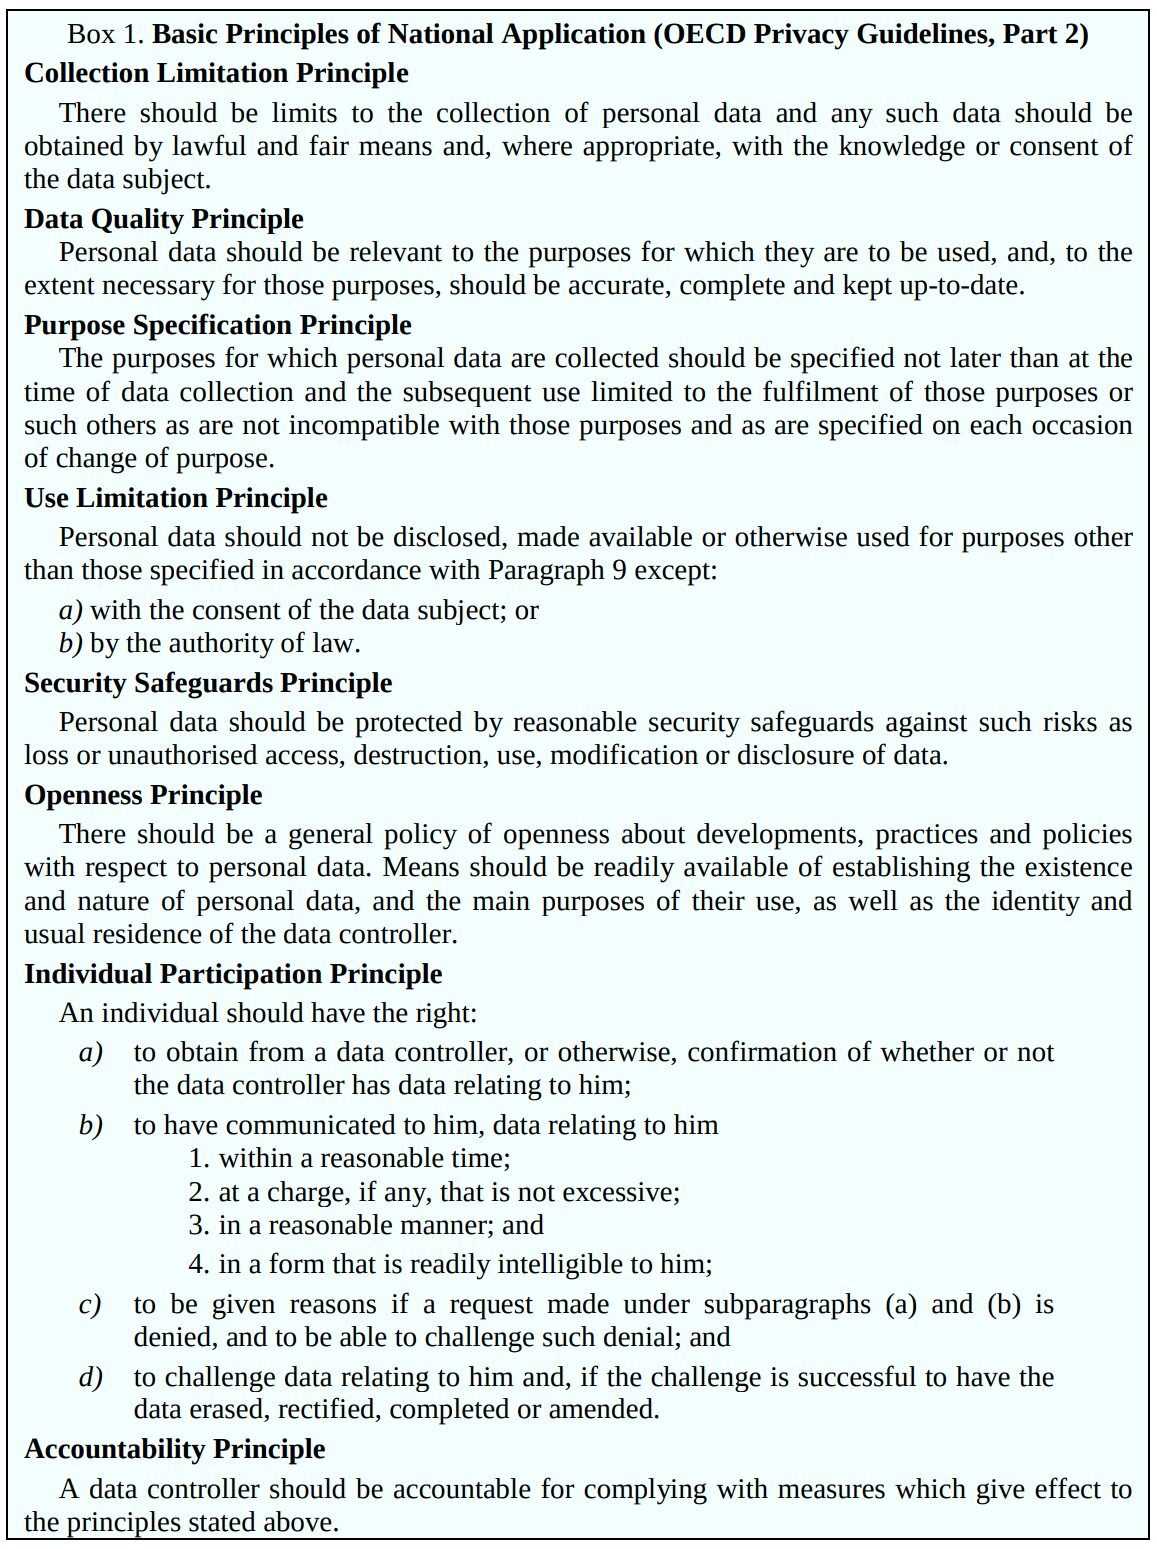
\includegraphics[width=\textwidth]{latex/figures/oecd_guidelines.jpg}
            \caption[OECD guideline]{OECD guideline \cite{oecd_oecd_2013}}
            \label{fig:oecd_guide}
        \end{figure}
        The first principle is the Collection Limitation Principle. It states that "There should be limits to the collection of personal data [..]" \cite{oecd_oecd_2013}. This principle is reflected in NIST's \textit{Guide to protecting the confidentiality of Personally identifiable information} \cite{mccallister_guide_2010}. In there, it is recommended to minimize the use, collection, and storage of personal data to the minimum necessary to serve its purpose.
        That way, the damage done on a possible data breach is minimized. It is also recommended to review the previously collected PII. If it is no longer relevant, it should be removed \cite{mccallister_guide_2010}.\\
        To protect data sets, the NIST guide also recommends the de-identification of information. Data with enough PII removed or obscured is treated as de-identified. One-way cryptographic functions (hash functions) may be used for this purpose \cite{mccallister_guide_2010}.\\
        Suppose there is no code or other association to re-identify the information is defined as anonymized \cite{mccallister_guide_2010}. This matches with the definition of anonymity and anonymization.


    \newpage
    %
    %%%%%%%%%%%%%%%%%%%%%%%%%%%%%%%%%%%%%
    %%%%%%%%%%%% Subsection %%%%%%%%%%%%%
    %%%%%%%%%%%%%%%%%%%%%%%%%%%%%%%%%%%%%
    %
    \subsection{Regulations}
        \label{subsec:related:law}
        Anonymity is defined by DIN EN ISO/IEC 29100 as an information characteristic that does not allow the identification of a person directly or indirectly \cite{german_institute_for_standardization_din_2020}. It furthermore declares anonymization as a process in which personally identifiable information is irrevocably transformed. This transformation denies the ability of an entity to identify a person indirectly or directly by itself or in cooperation with another entity \cite{german_institute_for_standardization_din_2020}.\\
        
        A major advantage of anonymized data is the exclusion of the GDPR legislation. Recital 26 of the regulation excludes anonymized data explicitly.\\ 
        "The principles of data protection should therefore not apply to anonymous information, namely information which does not relate to an identified or identifiable natural person or to personal data rendered anonymous in such a manner that the data subject is not or no longer identifiable. This Regulation does not therefore concern the processing of such anonymous information, including for statistical or research purposes." \cite{european_union_regulation_2016}\\
        Compared to the EU, the US have a wide range of privacy state laws. While the EU aims to provide one general regulation, the US privacy laws are split over four major regulations.
        These four are the \textit{Health Insurance Portability and Accountability Act} (HIPAA), \cite{rights_ocr_summary_2009}, which regulates healthcare provider, \textit{NIST 800-171} \cite{ross_protecting_2015}, which defines how to handle controlled unclassified information in non-federal information systems, the \textit{Gramm-Leach-Bliley Act (GLBA)} \cite{noauthor_gramm-leach-bliley_2013}, protecting personal information stored by financial institutes and the \textit{Federal Information Security Management Act (FISMA)} \cite{carper_s2521_2014} in which the requirements are stated for federal agencies information security programs. On top of these, states have additional privacy laws, which may be up to the GDPRs protection, depending on the state \cite{andrada_coos_eu_nodate}.\\
        The European data protection regulation provides a strong set of rules. These may be aggravated by member state laws but not weakened. This allows for even stronger data protections in some European countries.
        
    %
    %%%%%%%%%%%%%%%%%%%%%%%%%%%%%%%%%%%%%
    %%%%%%%%%%%% Subsection %%%%%%%%%%%%%
    %%%%%%%%%%%%%%%%%%%%%%%%%%%%%%%%%%%%%
    %
    \subsection{Private Data Publication}
        \label{subsec:related:private_data_analysis}
    
        \subsubsection{\textit{k}-anonymity}
            \label{subsec:related:kanon}
            To avoid the identification of a user, based on the published data and its attributes, record linkage should not be possible. Therefore a system design should consider the so-called quasi identifier (QI). These quasi identifiers may allow to draw a connection between the data set and an external source \cite{sweeney_k-anonymity_2002}.
            If a set of attributes is contained in an external release that might contain PII and contained in a released data set, these sets of attributes are called quasi identifiers, as it allows the linkage between these two data sets.
            If a data set S has $QI_S$ associated with it, S satisfies \textit{k}-anonymity if each sequence of values S[$QI_S$] appears at least \textit{k} times. 
        	In addition, each sequence S[$QI_S$] needs to belong to a different user.
        	This does protect the data set against linking by using direct matching, as Sweeny proposes in  \cite{sweeney_k-anonymity_2002}.\\
            One of the shortcomings of \textit{k}-anonymity is that each tuple of attributes needs to belong to a different user, as Fung demonstrates in  \cite{fung_introduction_2011}, as they are possibly expose sensitive data otherwise.

        \subsubsection{\textit{l}-diversity}
            \label{subsec:related:l-div}
            In  \cite{machanavajjhala_l-diversity_2007} Machanavajjhala et al. shows that k-anonymity is susceptible to the two attack vectors: homogeneity and background knowledge.
            The homogeneity attack works on datasets with groups that lack diversity in sensitive attributes. The background knowledge attack on the other hand uses available knowledge in addition to the provided dataset that is not directly matched to attributes.\\
            Machanavajjhala et al. introduce the \textit{l-}diversity framework to counter these weaknesses by requiring that the values of a sensitive attributes are well represented in each group. \textit{l}-diversity is not intended to replace \textit{k}-anonymity, but to extend it and improve privacy that way  \cite{machanavajjhala_l-diversity_2007}.
            

        % differential privacy
        \subsubsection{Differential Privacy}
            \label{subsec:related:dif_privacy}
            Differential privacy (DP) is a property of the data access mechanism and unrelated to auxiliary information available \cite{dwork_algorithmic_2013}. 
            It promises that the addition or removal of a single dataset to an existing database does not affect the outcome of an analysis with a strong mathematical definition of privacy. A protection against privacy attacks like re-identification, record linkage, and differencing is mathematically provable provided  \cite{agrawal_differential_2008},  \cite{wood_differential_2018}. \\
            This guarantees that anyone will make the same inference about an individual's PII or private information whether the individual's dataset was included in the analysis or not \cite{wood_differential_2018}. Therefore making post-processing impossible as an analyst can not make the output less differential private without additional knowledge of the private database \cite{nguyen_understanding_2019}.
            
%%%%%%%%%%%%%%%%%%%%%%%%%%%%%%%%%%%%%
%%%%%%%%%%%%%%%%%%%%%%%%%%%%%%%%%%%%%
%%%%%%%%%%%%   SECTION   %%%%%%%%%%%%
%%%%%%%%%%%%%%%%%%%%%%%%%%%%%%%%%%%%%
%%%%%%%%%%%%%%%%%%%%%%%%%%%%%%%%%%%%%
\section{Data Transmission}
    \label{sec:related:data_transmission}
    %
    The Tor Project is probably the most known approach for anonymized data transmission over the Internet. Besides Tor, we will discuss different approaches to transmit data over a network. In \ref{subsec:related:overlay} the Tor and I2P overlay network are going to be discussed, followed by the domain name system in section \ref{subsec:related:dns}. 
        
        
    %
    %%%%%%%%%%%%%%%%%%%%%%%%%%%%%%%%%%%%%
    %%%%%%%%%%%% Subsection %%%%%%%%%%%%%
    %%%%%%%%%%%%%%%%%%%%%%%%%%%%%%%%%%%%%
    %
    %%%% Overlay Networks
    %
    \subsection{Overlay Networks}
        \label{subsec:related:overlay}
        %
        Several overlay networks provide different functionalities. Caching overlays enhance the serving of static content. Routing overlays provide different features for dynamic content than the underlying networks and security overlays, that improve the security of networks and can help mitigating distributed denial of service (DDoS) attacks \cite{pathan_overlay_2014}.\\
        Two overlay networks will be discussed. On the one hand, there is Tor \cite{dingledine_tor_2004}, on the other, I2P \cite{zantout_i2p_2011}. Both systems aim to enhance the anonymity of the internet by adding additional layers.\\
        Furthermore, additional protocols like P5 \cite{sherwood_p_2005} and Herbivore \cite{goel_herbivore_2003} have been reviewed. As they are similar to the presented solutions, but are less known or require additional implementation steps or infrastructure, they are not described in this section.
     
     
    %%% Tor %%%
    \subsubsection{Tor}
        The so-called Onion Routing used  by Tor is a distributed overlay network to anonymize TCP-based applications. On its path from sender to receiver, each step in the network only knows its predecessor and successor. Therefore information is layered and secured with symmetric keys, which are unwrapped at each step, like the layers of an onion.
        Tor provides perfect forward secrecy by negotiating session keys with each successive hop. If one hop gets compromised, after the keys are deleted, old traffic can't be decrypted \cite{dingledine_tor_2004}, \cite{borisov_shining_2008}.\\
        Tor requires additional work on the client site to configure and set up. 
        The network is operated by a wide variety of people and organizations.
        Thousands of relay nodes are used to route traffic from the origin to the receiver. It was in 2009 and is of today the biggest network designed for anonymity in operation \cite{edman_anonymity_2009}.
        Therefore it is independent of the collecting entity. Tors systems provide anonymity for the sender against the server and an attacker in most cases \cite{arma_one_2009},  \cite{poulsen_feds_2013}, \cite{samson_tor_2013}, \cite{herrmann_website_2009}.\\
        The use of the Tor network is free of charge. It is open source software, but connecting to it requires additional setup steps from the user. To route only traffic of one application through the Tor network, configuration files need to be adjusted and additional software installed. As the Tor network is spread around the globe and no path can, or should, be provided, delay and latency increase, if the tor network is used for all applications on the device. Also the available resources would be reduced for tasks that are not required to have an extended privacy protection.\\
    
    
    
    %%% I2P %%%
    \subsubsection{The Invisible Internet Project - I2P}
        I2P is an overlay network with privacy-by-design in mind intended to connect services within a closed network.
        Exit proxy servers are available but not recommended by the developer. Within the network, nodes can communicate in any way they want. I2P is free open source software and can be added to a regular web service to make it available on the closed network. Each network node has unidirectional inbound and outbound tunnels, and every node is visible on the network. However, the traffic of a node can not be seen by other network participants. The network is decentralized and uses distributed hash tables for a network database and contact information security \cite{i2p_intro_2014}.\\
        To contact another client, a message is sent out through its own outbound tunnel, trying to reach the other client's inbound tunnel. Each client can choose the tunnels' length to find a trade-off between latency and anonymity \cite{anoncoin_i2p_2018}.\\
        I2P requires additional software or setup steps on the client and server-side to access the network.\\
        
        
        
    
    %%% VPN %%%
    \subsubsection{Virtual Private Network - VPN}
        A VPN provides an encrypted connection from the user's system to an exit point, the VPN server. For further communication, the IP address of the VPN server is used. This may change the country of origin and prevent things like geoblocking or other restrictions imposed by the internet service provider \cite{microsoft_virtual_2009}.\\
        A VPN provides privacy against prying eyes in the path from the client to the VPN server. It also provides anonymity to the web service requested. Virtual private networks can be self-hosted, hosted by a for-free or paid provider. Additional steps, like configuration, are required on the user's end to use it.\\

    
    %%%%%%%%%%%%%%%%%%%%%%%%%%%%%%%%%%%%%
    %%%%%%%%%%%% Subsection %%%%%%%%%%%%%
    %%%%%%%%%%%%%%%%%%%%%%%%%%%%%%%%%%%%%
    %
    %%%% Special systems
    %
    \subsection{Special Systems}
        \label{subsec:related:special}
        There are already systems available that have been designed for anonymized data collection and transmission. 
        Two such systems currently in use by major open source web browsers are dissected below. In \ref{subsec:related:dns} the domain name system is discussed. It is usually not connected to anonymous data transmission but provides a reliable way to disconnect the sender's IP address from the DNS query.
        %
        
    %%% Prochlo %%%
    \subsubsection{Prochlo}
        Prochlo describes a system architecture for large-scale monitoring of software usage activities. The system uses an "Encode, Shuffle, Analyze" approach. Thereby data is encoded and encrypted on one side. It's also the encoder's objective to add noise and take care of the randomness of the collected data \cite{bittau_prochlo_2017}.\\
        Afterwards, the data is transmitted to a centralized shuffler. They are responsible for the masking of the data origin by removing metadata (IP address, order, and time of arrival).
        The data is held for a prolonged time and transmitted only when a single data item is hidden in a crowd of similar data items. Therefore shufflers need to be trusted entities and separated from the analyzer \cite{bittau_prochlo_2017}. To add further trustworthiness, they should be run by a third party. The aggregated and reordered data is sent out at random intervals to further increase the decoupling of the time of arrival and enhance the privacy of clients.\\
        After transmission, the data is decrypted, stored, and aggregated by the analyzer. 
        Added noise and fragmentation on the encoder side, as well as shuffling, may be sufficient to provide differential anonymity in this system.
        
        Prochlo is developed by Google and used by Chromium and, in modified form, by Brave.
        \begin{figure}[hb]
            \centering
            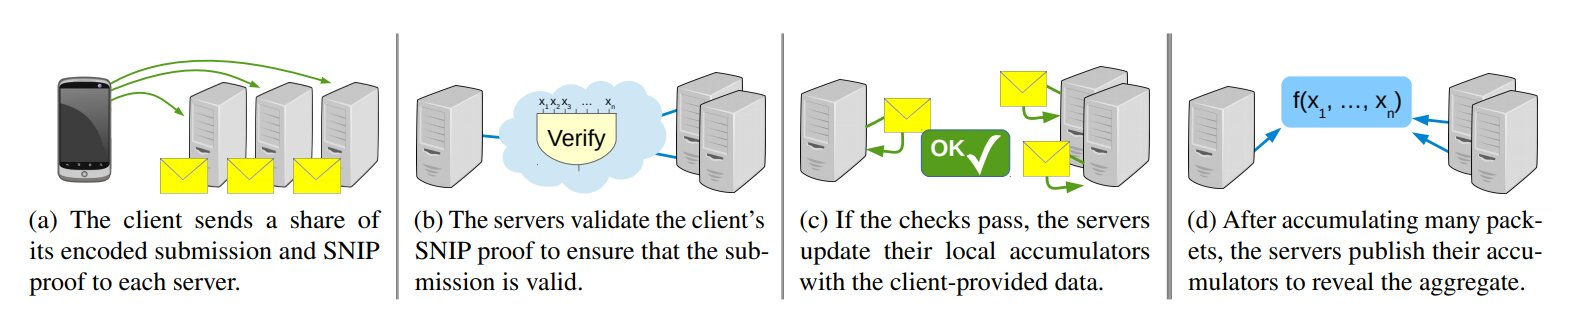
\includegraphics[width=\textwidth]{latex/figures/prio_overview.jpg}
            \caption[Overview of Prios processing pipeline]{Overview of Prios processing pipeline \cite{corrigan-gibbs_prio_2017}}
            \label{fig:prio_overview}
        \end{figure}
    
    %%% Prio
    \subsubsection{Prio}

        Prio was developed by Corrigan-Gibbs et al. \cite{corrigan-gibbs_prio_2017} in 2017 as a privacy-preserving system for collecting aggregated statistics.
        It was developed at Stanford University's Computer Science department for nonsensitive data already covered by their Telemetry tool. 
        Prio splits the collected client data into shares. 
        The parts are sent to different servers and aggregated with shares of other users before being published (see figure \ref{fig:prio_overview}) \cite{corrigan-gibbs_prio_2017}.\\
        The system promises privacy as long as one of the servers is honest, therefore providing strong cryptographic privacy. A limited form of robustness is provided as long as all servers are honest. It can detect and discard syntactically incorrect client data while preserving the privacy of the data. However, Prio can not prevent a client from sending in-range data, that is untrue \cite{corrigan-gibbs_prio_2017}.\\
        It is in experimental use by Firefox Origin Telemetry \cite{englehardt_next_2019}.
        
        
    %%% DNS 
    \subsection{Domain Name System - DNS}
        \label{subsec:related:dns}
        The Domain Name System is hierarchically and decentralized designed to allow systems connected to a network to translate memorable domain names into IP addresses \cite{stevens_tcpip_1993}.\\

        This translation is needed before an application can request a TCP connection or send UDP datagrams. A domain name is a list of labels separated by dots. 
        Each label can have a length of up to 63 bytes, with a maximum length of the requested domain of 255 bytes \cite{stevens_tcpip_1993}.\\
        The dot is used to separate each layer in a domain but is also the internet root, which terminates all Fully Qualified Domain Names (FQDN), but is often omitted \cite{jeftovic_managing_2018}.
        In figure \ref{fig:dns_tree} it is shown how a hostname can be separated and traversed.
        The first field, following the, here omitted, root entry is the so-called Top-Level Domain (TLD). In figure \ref{fig:dns_tree} this would be "com". The root and top-level domain are required to find the responsible authoritative nameserver for any related query \cite{jeftovic_managing_2018}.

    	\begin{figure}[h!]
    	    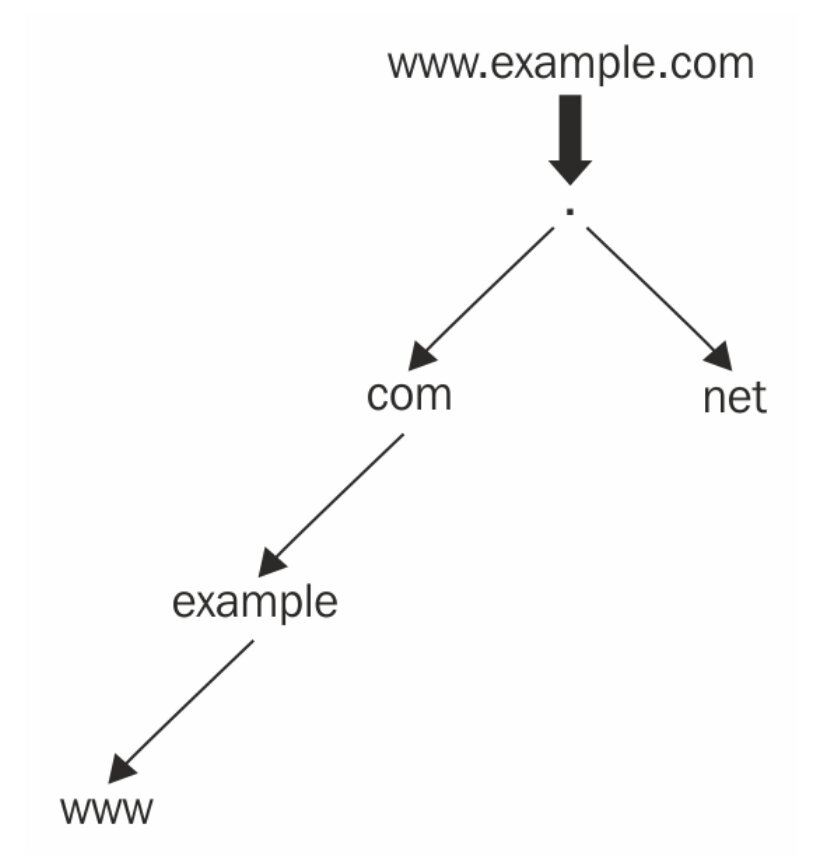
\includegraphics[width=\textwidth]{latex/figures/domain_name_tree.jpg}
    	    \caption[Domain Name Tree for www.example.com.]{Domain Name Tree for www.example.com. \cite{jeftovic_managing_2018}}
    	    \label{fig:dns_tree}
        \end{figure}

        The name system is structured in non-overlapping zones, as shown in the right segment in figure \ref{fig:dns_query} with the root domain on top \cite{herrmann_beobachtungsmoglichkeiten_2016}.
        A server containing all information about a subset of the namespace is called an authoritative server. To extract the information from the authoritative server, a so-called resolver is used \cite{friedewald_privacy_2018}.
        As the hierarchical structure of the domain name system provides sender anonymity, meaning the receiver does not know the source of the message, the system can be used to transmit data anonymously to a collecting server. This can be achieved without any further additions to the protocol or configuration on the client-side.
        Advanced techniques like DNS over HTTPS (DoH) \cite{ermert_cloudflare_2020} \cite{mcmanus_dns_2018} or DNS Security Extensions (DNSSEC) \cite{larson_dns_2005} can be used.\\
        DoH uses transport layer security (TLS) to encrypt a connection to a proxy server, which then transmits the DNS request. That way, the proxy server is the only participant who knows the sender's IP address. DNSSEC can add another layer of security in protecting against attacks like DNS cache poisoning by adding new components to the DNS system that check the integrity and authentication of DNS data.\\
        The newly presented Oblivious DNS over HTTPS (ODoH) developed by Apple, Fastly, and Cloudflare may add additional privacy to every DNS query and removes one weakness from DoH \cite{verma_improving_2020}.\\
        In ODoH, the client encrypts its DNS request for a target server and sends this encrypted message to the proxy server, which then relays the message to the target server. This procedure removes the original request from the client's IP, making the proxy unaware of it.
        At the same time, the target server only knows the IP of the proxy as the source. The response is then encrypted for the client and relayed back through the proxy \cite{verma_improving_2020}.
        
        
        
        %%% TODO: citation for DOH and DNSSec
        
        \begin{figure}
            \centering
            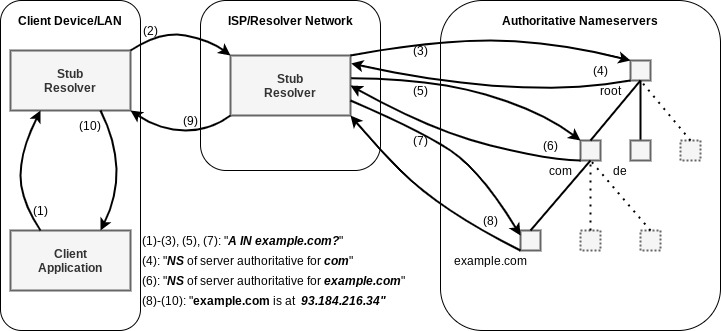
\includegraphics[width=\textwidth]{latex/figures/dns_resolve.jpg}
            \caption[DNS Query with resolver for example.com]{DNS Query with resolver for example.com, based on \cite{friedewald_privacy_2018}}
            \label{fig:dns_query}
        \end{figure}
        
        
        The DNS is also used in malware for DNS tunneling or data exfiltration.
        In DNS tunneling domain TXT records are used to initiate a session with a command and control server. The TXT field can also contain instructions for the malware \cite{das_detection_2017}.\\
        To exfiltrate data in a DNS request, the information in question is Base32 encoded and split into 63 byte sized chunks. Afterwards, requests are started to a monitored or controlled domain with the encoded data as fields \cite{mertens_infosec_2017}.\\
        
\newpage
%%%%%%%%%%%%%%%%%%%%%%%%%%%%%%%%%%%%%
%%%%%%%%%%%%%%%%%%%%%%%%%%%%%%%%%%%%%
%%%%%%%%%%%%   SECTION   %%%%%%%%%%%%
%%%%%%%%%%%%%%%%%%%%%%%%%%%%%%%%%%%%%
%%%%%%%%%%%%%%%%%%%%%%%%%%%%%%%%%%%%%
\section{Related Software}
    \label{sec:related:related_sw}
    %
    This section introduces some open source projects that allow data collection or actively collect user-system information. 
    
    %%% Ubuntu %%%
    \subsection{Ubuntu}
        Ubuntu is one of the best-known distributions of the GNU/Linux Operating system. It provides several packages for server, desktop, or embedded usage. It is used by many major companies on their server \cite{canonical_enterprise_nodate}\\
        Ubuntu collects data with its "ubuntu-report" tool. By default, a system reports its data only once per distribution version. The tools provide a graphical user interface and command-line version and prompt the user's information before sending \cite{roche_ubuntuubuntu-report_2020}.\\
        A JSON report, as shown in listing \ref{lst:ubuntu-report} in the Appendix, is sent to the Ubuntu server if the user opts in. If the user opts out, a report is created as in listing \ref{lst:opt-out} and sent to the Ubuntu server \cite{roche_ubuntuubuntu-report_2020}.\\ 
        \begin{lstlisting}[language=json, caption=JSON report on opt out, label=lst:opt-out]
            {
                "OptOut": true
            }
        \end{lstlisting}
        This allows Canonical to get a relatively precise number of internet-connected devices that run Ubuntu.\\
        There is no PII collected. Only data like system architecture, RAM, disk space, monitor count, and resolution are reported.\\
        An HTTP POST is sent over TLS to the Ubuntu server to transmit the data.\\
        
        In an HTTP POST, the body of the message contains the payload, compared to a GET, where the payload is appended to the URL.
        It is not encrypted or encoded by default but can be upfront to protect the body's data from inspection. Protocols like TLS can be used to encrypt the transport. But if an attacker knows the session key, all ongoing communication can be read. Prior communication is secured as TLS provides forward secrecy.\\
        
        As this is a TCP direct connection, the public IP address of the sending system can be connected to the collected data on the server-side.
        The user must trust the collecting services, that the information is not stored but discarded.\\
        
    %%% hw-probe %%%
    \subsection{Hardware Probe Tool - hw-probe}
        The Hardware Probe Tool is an open source tool to collect hardware, system, and log information on Linux and BSD-based systems. It is written in Perl, and collected data is available for everyone to see. 9780 unique systems reported their system information in 2019 \cite{ponomarenko_linux_nodate}.
        While serial numbers and MAC addresses are collected, they are salted and hashed with SHA512, and only 32 bytes are transmitted. With salting, additional (random) data is added to the original message to increase the effort for reidentification attacks.
        This should avoid the recreation of any personal identifiable information and uniquely identify a system against the database  \cite{project_linuxhwhw-probe_2020}.\\
        The collected data can be pretty extensive if a complete collection is enabled. It includes, among other things, installed drivers, connected PCI devices, system architecture, operating system, network interface type, and UUID \cite{project_linuxhwhw-probe_2020}.\\
        
        HTTP POST messages are sent to the collection server to transmit the collected data. The transmission uses TLS to secure the content of these messages \cite{project_linuxhwhw-probe_2020}.\\
        Again the IP of the system is connected to the data set transmitted, and the user has to rely and trust on the collecting entity to separate this two information from each other.\\
    


\newpage
    %%% Firefox %%%
    \subsection{Firefox}
        Firefox is a browser that promises speed and privacy. It provides advertisement and tracker blocking. Besides, it is available on all major platforms \cite{mozilla_corporation_download_nodate}.\\ 
        By default, Firefox collects a wide range of data. These data collections are called Pings. Each Ping contains a certain type of information. There are at least 27 different Ping types in use at the time of writing \cite{mozilla_telemetry_nodate}.
        
        \begin{wrapfigure}{R}{0.41\textwidth}
            \centering
            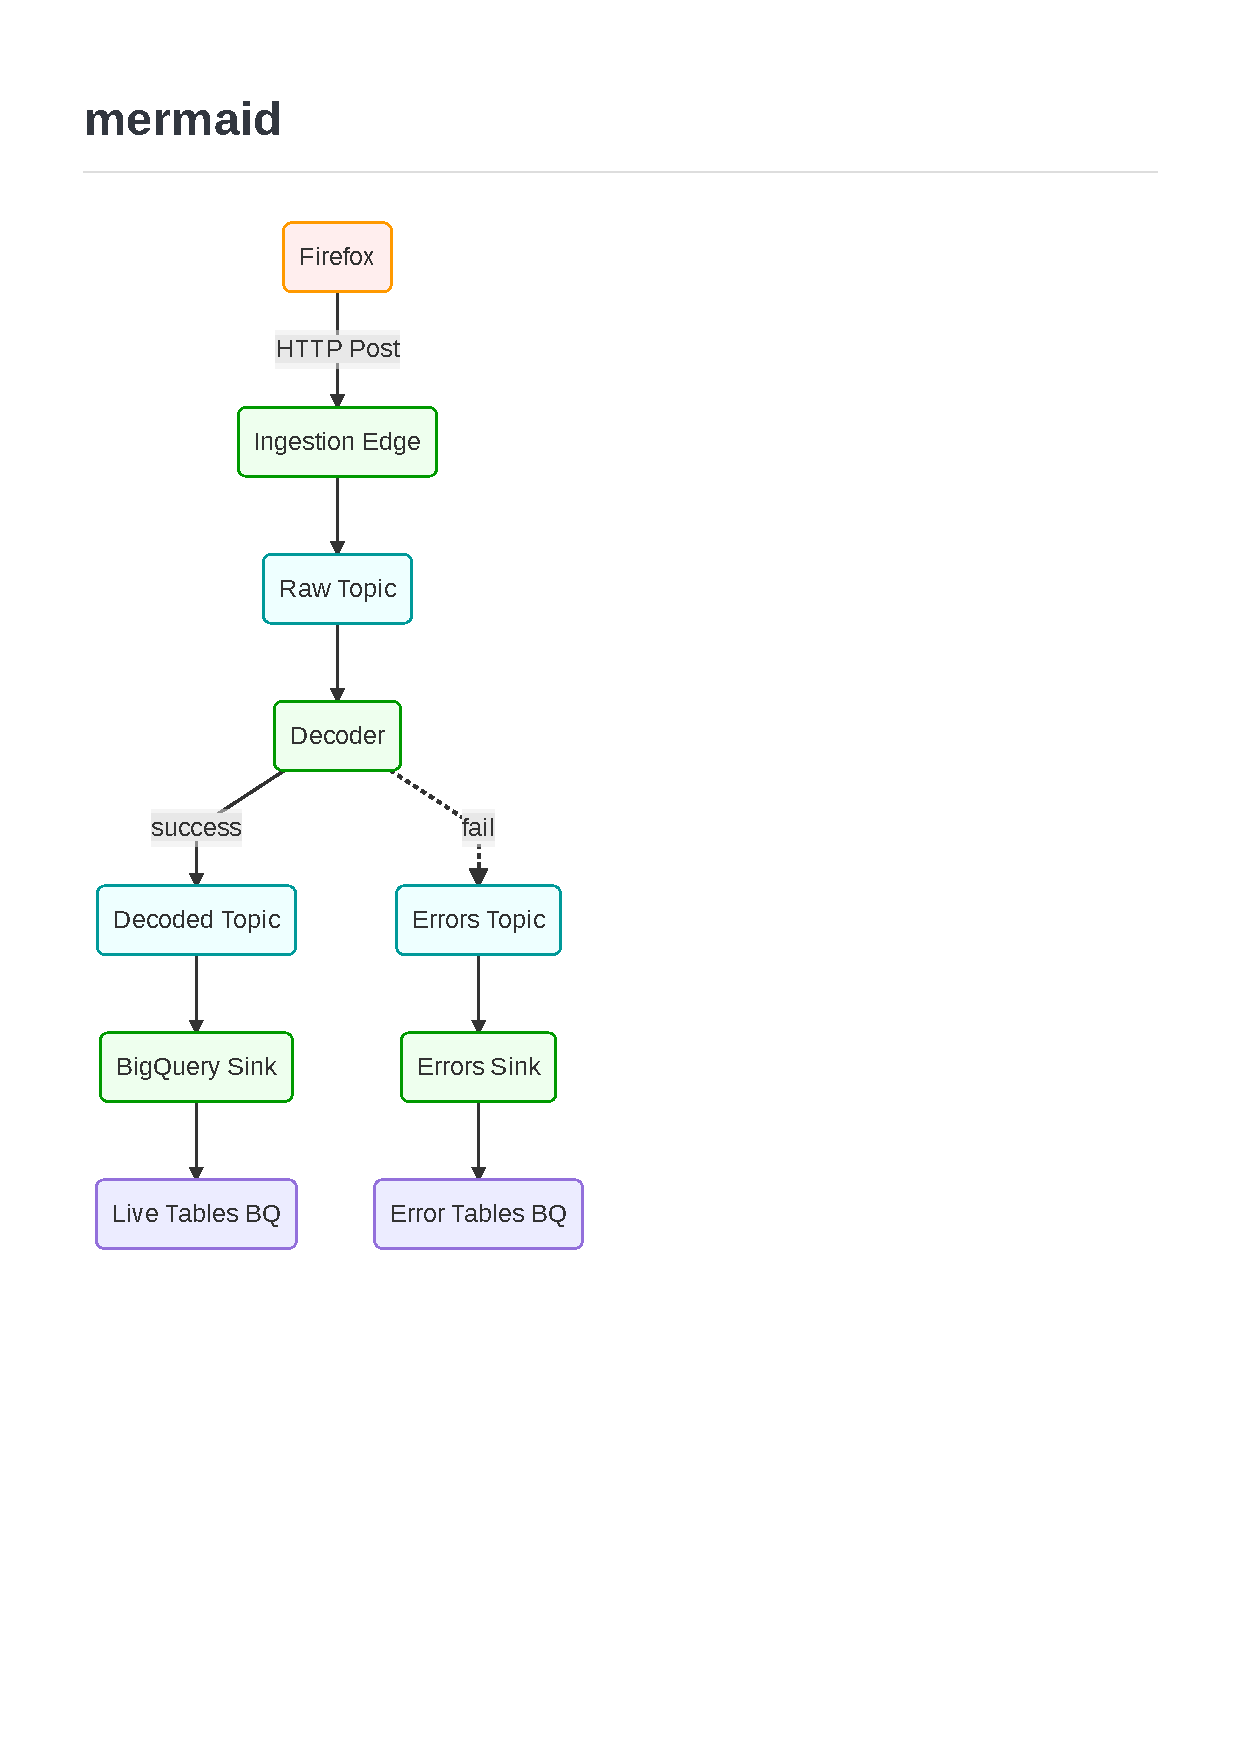
\includegraphics[clip, trim=0.5cm 8cm 8cm 3.5cm, width=0.4\textwidth]{latex/figures/firefox_telemetry_graph}
            \caption[Firefox data flow]{Firefox data flow based on  \cite{mozilla_overview_2020}}
            \label{fig:moz_data_flow}
        \end{wrapfigure}
        
        The "main" Ping is used for most telemetric data. It contains extensive health and performance information on Firefox, but also most system information. The JSON structure of a "main" Ping can be seen in Mozillas pipeline schema GitHub repository \cite{mozilla_mozilla-servicesmozilla-pipeline-schemas_2020}. 
        Besides information on CPU, GPU, and operating system, it contains information on installed add-ons and the reason for sending the Ping.
        It is sent at least every 24 hours, but also on startup and other occasions. While basic telemetry, like the main ping, can be disabled on the settings page, Firefox will still send selected Pings to its server unless disabled in \textit{about:config}.
        %TODO: verify with wireshark - firefox sends stupid amount of data
        To send the collected Telemetry, Firefox uses a program called Ping Sender.
        This will send an HTTP POST to the Edge Server, where it is forwarded to the data pipeline, if formatted correctly.
        If a client IP address is available at the decoder, the geolocation will be determined and saved.
        The IP address gets discarded from the data set in the process \cite{mozilla_overview_2020}, \cite{mozilla_http_2020}, \cite{firefox_ping_nodate}.\\
        A reduced data pipeline can be seen in figure \ref{fig:moz_data_flow}.
        
        
        
    
        Mozilla was experimenting with Prio in 2018, \cite{helmer_testing_2018}, and based on the experiment they developed Firefox Origin Telemetry  \cite{englehardt_next_2019} which is, at the time of writing, in use only for content blocking and still experimental \cite{noauthor_origin_nodate}.\\
    
    
    %%% Brave %%%
    \subsection{Brave}
        Brave is a free open source browser with a focus on privacy. It provides advertisement and tracker blocking, as well as a Tor integration. It is based on Chromium and promises to be faster. It also claims to have better default privacy than Firefox. It is a relatively new Browser but already supports all major platforms \cite{brave_secure_nodate}.\\
        Brave uses a technique called Privacy Preserving Product Analytics (P3A) for telemetry data, which can be turned off at any time.
        They claim that their P3A does cover way more than expected by GDPR. No personally identifiable data (PII) is collected or transmitted \cite{brave_privacy-preserving_2019}.\\
        Therefore Braves telemetry process is split into two phases. The first phase consists of several multiple-choice questions, for which the answer is sent individually.
        Each question poses a number of answers. Quantifiable questions, like the number of open tabs, provide ranges for each answer for enhanced privacy \cite{brave_privacy-preserving_2019}. These Questions and possible answers can be reviewed in Braves GitHub repository \cite{brave_software_inc_brave-browser_2019}.
        The questions of phase one can be seen in listing \ref{lst:brave-report} in the appendix.\\
        At a randomized time after opening the browser, the number of open tabs is counted and send out once an hour with further information \cite{brave_privacy-preserving_2019}.
        An answer contains:
        \begin{itemize}
            \item Question number, Answer number
            \item OS/Platform
            \item Release information (nightly/dev/bet/release)
            \item Week of installation (if the installation was within 90 days)
            \item Country (if fewer than 6000 installs per week, this is removed)
            \item Referral code (only if within 90 days of install and referrer is big enough)
        \end{itemize}
        Every answer is sent to Braves content delivery network (CDN) and stripped of the IP address of the client at the edge of the CDN \cite{brave_privacy-preserving_2019}.
        . 
        The Second Phase uses a protocol based on Prochlo (see \ref{sec:related:data_transmission}). 
        
        The study Leith conducted in February 2020  \cite{leith_web_2020} supports the claims made by Brave for a privacy caring browser.\\
        In his survey, Leith evaluated the privacy settings of six browsers (Brave, Chrome, Edge, Firefox, Safari, and Yandex). While Brave and Firefox (with changed defaults) were strongly focused on privacy, all Browsers did send their reports combined with the user's IP address \cite{leith_web_2020}.
        This is problematic, as an IP address can be used to pin down the user's geolocation \cite{koch_geolocation_2013}. Workplaces or homes can be derived based on the time people spend in places during the day or night. 
        While Brave Software Inc. claims that they remove the IP address at the edge of their CDN, the user has to trust the CDN operator to strip the send data of the address for phase one answers. In phase two, the user has to trust the shuffler to remove the metadata from the collected data. 
\newpage

%%%%%%%%%%%%%%%%%%%%%%%%%%%%%%%%%%%%%
%%%%%%%%%%%%%%%%%%%%%%%%%%%%%%%%%%%%%
%%%%%%%%%%%%   SECTION   %%%%%%%%%%%%
%%%%%%%%%%%%%%%%%%%%%%%%%%%%%%%%%%%%%
%%%%%%%%%%%%%%%%%%%%%%%%%%%%%%%%%%%%%
\section{Summary}
    In this chapter, we discussed what personal information is and how it should be handled.
    In addition, we summarized previous work on related topics. This allows us to narrow our research.
    Prio and Prochlo require additional infrastructure. As open source organizations are usually underfunded, every additional server leaves a dent in the budget. Therefore these systems may be
    useful for organizations with sufficient funding, but not for small projects. Some of the mentioned systems in this chapter depend on the user's trust that their transmission information is stripped from the data.\\
    
    On the other hand, client-side enabled anonymization, like using the tor network or VPNs, may require additional maintenance or knowledge from the user. This could reduce the amount of participating users significantly.\\
    
    The Domain Name System provides a hierarchical structure that strips the sender's information from the transmitted data in a reliable way. A user can trust the DNS to remove its IP and does not depend on an organization to handle that properly. Furthermore the anonymization process does not require any additional knowledge.\\
    Utilizing DNS for data transmission opens up a range of new issues, like plain text data transmissions. These issues need to be handled and will be discussed in the next chapter.\\ 

%


  
%%%%%%%%%%%%%%%%%%%%%%%%%%%%%%%%%%%%%%%%%%%%%%%%%%%%%%%%%%%%%%%%%%%%%%%%%%
%%%%%%%%%%%%   CAPTER 3   %%%%%%%%%%%%%%%%%%%%%%%%%%%%%%%%%%%%%%%%%%%%%%%%
%%%%%%%%%%%%%%%%%%%%%%%%%%%%%%%%%%%%%%%%%%%%%%%%%%%%%%%%%%%%%%%%%%%%%%%%%%
\chapter{Software Design}
\label{chap:software_design}

As mentioned in the previous chapter, we are going to focus on the challenges faced when utilizing the domain name system. Before we discuss the transport of data through the hierarchical name system in section \ref{sec:software_design:tx}, we will have at look at the data collection and ID generation (\ref{sec:software_design:data_collection}).\\
Section \ref{sec:software_design:ref_impl} demonstrates how we realized the proposed solutions in the reference implementation.

%%%%%%%%%%%%%%%%%%%%%%%%%%%%%%%%%%%%%
%%%%%%%%%%%%%%%%%%%%%%%%%%%%%%%%%%%%%
%%%%%%%%%%%%   SECTION   %%%%%%%%%%%%
%%%%%%%%%%%%%%%%%%%%%%%%%%%%%%%%%%%%%
%%%%%%%%%%%%%%%%%%%%%%%%%%%%%%%%%%%%%
%\section{Parameter}
%\label{sec:measurement:parameter}

%

%\newpage


%%%%%%%%%%%%%%%%%%%%%%%%%%%%%%%%%%%%%
%%%%%%%%%%%%%%%%%%%%%%%%%%%%%%%%%%%%%
%%%%%%%%%%%%   SECTION   %%%%%%%%%%%%
%%%%%%%%%%%%%%%%%%%%%%%%%%%%%%%%%%%%%
%%%%%%%%%%%%%%%%%%%%%%%%%%%%%%%%%%%%%
\section{Data Collection}
\label{sec:software_design:data_collection}
    As we have shown in \ref{subsec:related:pii} and \ref{subsec:related:law} it is wise to avoid the collection of PII. While it may be avoidable for the statistical data and numeric values, this might not be possible for the generated ID.\\
    The ID should be unique to identify a device persistent over reboots and system updates, but don't allow to draw conclusions on a device.
    While the gathered data needs to be useful to the purpose of the collection, the collection practices need to be compliant to the according privacy laws as well. 
    
 %
    %%%%%%%%%%%%%%%%%%%%%%%%%%%%%%%%%%%%%
    %%%%%%%%%%%% Subsection %%%%%%%%%%%%%
    %%%%%%%%%%%%%%%%%%%%%%%%%%%%%%%%%%%%%
    %
    \subsection{Data selection}
        \label{subsec:software_design:selection}
        To get the most out of data collection it needs to be relevant to the task it has to fulfill.
        While a wide range of collected metrics might help to broaden the view over the landscape that is monitored, it may hinder in the evaluation and detection of relevant data points. Therefore data collection should always be kept to a minimum needed to help the cause for the collection.\\
        In addition user are more willing to share non sensitive information as Woldaregay et al. \cite{woldaregay_user_2020} have shown for medical data, Ziefle et al.\cite{ziefle_users_2016} for data sharing on social networks and Leon et al. \cite{leon_what_2013} for sharing information with online advertiser. Furthermore Schneegrass et al. \cite{10.1145/3290605.3300753} have shown, that the willingness of information sharing for sensory data is based on a positive or negative connotation of the data in question.\\
        
        As we discuss Internet connected data collections, there is always the possibility for a data breach, or an adversary actor, who may target the collected data. If PII is contained in the data set, the possible yield for an attacker is higher, compared to public non personal identifiable data.\\
        To protect the devices and thereby the users identity, numerical data should always be collected in bins or ranges.\\
        The exact amount of available memory in a system provided in byte or even kilobyte may fingerprint a device. IP and MAC addresses are sensitive data as well and should not be collected at all, as these could be connected to other Internet related activities and lead to an attack on the user, to gain control over their device. \\
        As the National Academies of Science, Engineering and Medicine propose in their Consensus report \cite{groves_federal_2017}, the more attributes are included in a data set the likelier the re-identification of individuals and the greater the threat for external data linking.\\
        
        Prior to collecting data large scale a project should define the intend behind the process. With a clear outline of objectives, relevant parameters can be identified 
        Therefore we propose a minimal data collection set containing only information that are relevant to fulfill the purpose of the collection as recommended by NIST and OECD.\\
        To be open about the collected information, the current state of the collection should be easily available to any user, as well as the reasoning for the collection of each date.
        Following NISTs recommendations again, these data sets should be reviewed on a regular basis, to validate that each date is still needed.\\
        
        The objective for an open source project could be to reduce the amount of defects in the released software, or  to collect usage statistics to improve the development of the software for a given target. A combination of objectives is possible as well.\\
        Based on the objectives, a list of parameter can be compiled to retrieve data relevant to the purpose.
        To e.g. detect system crashes, the time since last reboot (uptime) of a given device may be relevant, as well as the amount of memory available and the CPU/SoC. Further on, the software version in use needs to be included in this example. These are all non-PII and may be collected without further obfuscation. As we have stated before, it is recommended to 
        classify numeric values, like available memory into categories.\\
        
        Although the collected information don't need to be obfuscated, the user should be made aware of the data collection. In some cases the users acknowledgment might be required as well. Therefore banner, push notifications or notifications on installation or first execution should be shown to the user. \\
        In case of a Linux distribution this could be done by a pop up message on first login to graphical screen or using a banner on a remote or serial login to the device.
        The GDPR requires that consent must be given specifically and may be withdrawn at any time\cite{noauthor_gdpr_2020}.\\ 
        Therefore a Linux distribution might require to click or set a value to enable and disable the data collection. An IoT firmware, like Tasmota might need to enable data collection via a web interface for a device. This needs to be done, before any user information is collected\\ 
        
        Furthermore an organization should provide a privacy policy for the data collection, even if no PII is collected. It should state which information is collected and transmitted on a given device.\\
        This could be seen as good faith and increase the users trust in in the data collection program. If private information is collected a privacy policy is required be GDPR. Another important point to be compliant is the right to be forgotten. This makes an identifier an important factor to recognize the users data. It needs to be available to the user, to exert her right to remove the data from a collection.
        
          
    \subsection{ID generation}
        \label{subsec:software_design:id}
        To keep the actions required by user to participate to the minimum feasible, ID generation should be an automated process without the need for the user to register for data collection. There are some registration processes available like Kluczniak et al. show in \cite{kluczniak_anonymous_2015} that provide a robust way to separate the user data from the token used to sign-up. But this would require the user to actively register for the collection process, which would most likely reduce the number of user participating.\\
        
        To identify devices on a reliable and reproducible basis the ID generation is based on hardware information available and is therefore persistent through a reboot, a re-flash or an update.\\
        We recommend the use of the available MAC-addresses. These should be hashed individually and and combined into one string which is then hashed again. Both hashing operations should be done with a strong cryptographic hashing function.
        As there are several different hash functions out there, the hashing should be one way and un-keyed. A one way hash function (OWHF) fulfills the requirements for a hash \textbf{\textit{h}} function, which can be seen in equation \ref{eq:hash}\cite{sobti_cryptographic_2012}.
        
        \begin{equation}
            \label{eq:hash}
            \textbf{h} : D \longrightarrow R
        \end{equation}
        
        where domain $D = \{0,1\}^*$ and $R=\{0,1\}^n$ for $n >= 1$.
        
        In Addition an OWHF must meet five requirements defined by Merkle in \cite{merkle_secrecy_1979}.
        \begin{itemize}
            \item \textbf{\textit{h}} must be applicable to any length of data blocks
            \item A fixed length output is created by \textbf{\textit{h}}
            \item A message digest \textbf{\textit{h}}(x) with \textbf{\textit{h}} and x given is easy to compute
            \item If \textbf{\textit{h}} and \textbf{\textit{h}}(x) are known, it is computationally infeasible to find x
            \item If \textbf{\textit{h}} and \textbf{\textit{h}}(x) are known, it is computationally infeasible to find x and x' so that $\textbf{\textit{h}}(x) = \textbf{\textit{h}}(x')$
        \end{itemize}
        
        This function should come from the Secure Hash Algorithm 2 or 3 (SHA-2/SHA-3) family. While SHA512 is the stronger function and is recommended, it is not available on all devices.\\
        A single MAC consists of 48 bit, from which 24 bit are a vendor specific and equal over all devices from this vendor. The other 24 bit are a unique identifier for a given network interface. As most internet connected devices come with pre-installed/soldered network interfaces, this could lead to brute force attempts to regenerate the MAC-address from a hash. Especially on hardware with only one physical network interface. With the power jump in recent graphic card generations a hash that is only based on 24 unique bits can be brute forced in very short time. Therefore the generated hash needs to be enhanced.\\
        
        There are some will known ways to enhance security on stored passwords and similar tasks. Three of them are PBKDF2\cite{kaliski_pkcs_2000}, Bcrypt\cite{provos_future-adaptable_1999} and Scrypt\cite{josefsson_scrypt_2016}.
        Bcrypt is a key derivation functions (KDF) based on the Blowfish block cipher. It receives a number of inputs, like iteration count, input password and salt. The password is limited to 56 bytes and the iteration count \textit{n} results in $2^n$ bcrypt iterations. It is designed to be secure through to be memory and storage complex\cite{hatzivasilis_password_2015-1}\cite{provos_future-adaptable_1999}.\\
        Scrypt is also a password based key derivation function which was designed to be computational complex to increase the costs of hardware based attacks. It creates a key from a list of inputs, that define the cost of the function.\\
        These key derivation functions have two use cases. On the one hand they are used for password hashes in modern operating systems, protecting the users password against easy access\cite{percival_stronger_nodate}. 
        The other use case is the derivation of a key based on a token and another key\cite{camenisch_privacy_2011}. Attacking a KDF in itself is not feasible. An attacker would need to iterate over a range of passwords or regular expressions and apply the KDF to them\cite{percival_stronger_nodate}.\\
        Another example of such a derivation function is Password-Based Key Derivation Function 2 (PBKDF2), in which a pseudo-random function is applied to a given password and salt for a number of iterations. 
        Salting reduces it's vulnerability against brute force and dictionary attacks attacks in which an adversary either starts guessing passwords and applies the function to it's guesses, or uses a set of rules or words from a list. Rainbow table attacks, which utilizes precompiled hash tables are made less feasible with salting as well and the computation time is increased significantly\cite{kaliski_bkaliskirsasecuritycom_pkcs_2000}. \\
        While Scrypt is designed to be an expensive function to break for an attacker, it is also the most resource demanding function during the creation of the key, reducing it's usability for embedded devices. Bcrypt is also computational intense and therefore resistant against attack from ASICs or GPUs. PBKDF2 is only a small circuit implementation and requires the lowest amount of RAM, which makes it best suited for embedded devices, while reducing it's effectiveness against brute force attacks on ASICs or GPUs\cite{hatzivasilis_password_2015-1}.\\

        To keep IDs reproducible we need to derive our input password and salt from data provided by the device, which wont alter during a reinstall of a system. For devices with non volatile flash memory the Memory Technology Devices (MTD) are usually devices with solid state file systems\cite{giometti_mtd_2017}\cite{woodhouse_memory_nodate}. These partitions can contain configuration information for wireless devices. This contains device-unique data which is ideal to use as key and/or salt.\\
        
        To further strengthen the ID against brute forcing and decreasing the amount of character used in a DNS query, the generated ID should be reduced to feasible number of bytes. Hereby the number of expected user should be in relation to selected byte length of the ID.\\
        The available numbers of variation may be calculated for given string length \textit{n} and length of alphabet \textit{k} as seen in equation \ref{eq:variations}.
        \begin{equation}
            \label{eq:variations}
            V(n;k) = n^{k}
        \end{equation}

        As DNS limits the available alphabet to [a-z][0-9] this would fix \textit{k} to $26 + 10 = 36$.
        
        To calculate the probability of a hash collision, we can utilize equation \ref{eq:base_prob_hash}
        
        \begin{equation}
             \label{eq:base_prob_hash}
             P(k,V) = 1 - \exp{\frac{-k(k-1)}{2 * V}}
        \end{equation}
     
        Based on \cite{preshing_hash_2011} equation \ref{eq:base_prob_hash} can be simplified for expected collisions probabilities of $\frac{1}{10}$ or less and large k to
     
        \begin{equation}
            \label{eq:simp_prob_hash}
            P(k,V) = \frac{k^2}{2V} 
        \end{equation}
        
        The generated IDs should have a low collision probability rate to keep them unique, but should be selected small enough, to keep the bytes used in a DNS request low. \\
        To calculated a possible number of hashes, with a given probability \textit{P} we can transform equation \ref{eq:simp_prob_hash} to a reduced quadratic equation
        \begin{equation*}
            0 = k^2 - 2PN
        \end{equation*}
        which can then be solved as seen in equation \ref{eq:solvek}
        \begin{equation}
            \label{eq:solvek}
            k = \sqrt{2PN}
        \end{equation}
        
        With equation \ref{eq:solvek} it is possible to calculate the amount of supported user/devices, before the risk for a hash collision reaches the threshold.
\newpage



%%%%%%%%%%%%%%%%%%%%%%%%%%%%%%%%%%%%%
%%%%%%%%%%%%%%%%%%%%%%%%%%%%%%%%%%%%%
%%%%%%%%%%%%   SECTION   %%%%%%%%%%%%
%%%%%%%%%%%%%%%%%%%%%%%%%%%%%%%%%%%%%
%%%%%%%%%%%%%%%%%%%%%%%%%%%%%%%%%%%%%
\section{Data Transmission}
\label{sec:software_design:tx}
%
    While the ID is generated in a way to be transmitted over DNS, the collected data is still in plain text and a large chunk of text. As we have shown in \ref{subsec:related:dns} only 63 byte long labels up to a total of 255 bytes for a complete request are supported.
    Therefore the data needs to encrypted, to provided privacy during the transport and chunked and transformed to allow a transport over DNS.\\
    %
    %%%%%%%%%%%%%%%%%%%%%%%%%%%%%%%%%%%%%
    %%%%%%%%%%%% Subsection %%%%%%%%%%%%%
    %%%%%%%%%%%%%%%%%%%%%%%%%%%%%%%%%%%%%
    %
    \subsection{Data Encryption}
        \label{subsec:software_design:encryption}
        To provide privacy and security to the client the collected data should never be transported unencrypted over the internet. An attacker might be able to monitor the DNS request send by the client and use the contained information to figure out possible weaknesses of the system in use from them and maybe available additional information. \\
        In comparison to the generated ID, where we rely on the irreversibility of the result, the encryption of the data needs to be reversible to perform statistical analysis on them.
        Again the load on the user should be minimal. Therefore we would recommend an automated system again.\\
        A well known system for secure data transport is TLS, which is used in modern HTTPS implementations. TLS utilizes asymmetric encryption, also known as public key encryption. 
        Thereby a publicly available key, the public key, is used to encrypt the data on one side by anyone. The private key on the other hand is usually only available at one instance, which decrypts messages encrypted with the public key. In TLS asymmetric cryptography is used in key exchange algorithms, to agree on session keys, which then in turn are used for symmetric encryption, once the session build up is complete\cite{noauthor_how_nodate}.\\
        As there should be no session build up between the client and the collecting server to keep the anonymity of the sender intact, we recommend asymmetric encryption.
        One of the most employed asymmetric encryption systems is the Rivest-Shamir-Adleman algorithm (RSA). They proposed procedures with the following four properties\cite{rivest_method_1978}.
        \begin{itemize}
            \item The encryption procedure \textit{E} and the decryption procedure \textit{D}, are both easy to compute.
            \item Only \textit{D} can decrypt messages encrypted with \textit{E}. When \textit{E} is published, there is no easy way to compute \textit{D} from it
            \item Deciphering an enciphered Message \textit{M} results in \textit{M}. \textit{D(E(M)) = M}
            \item \textit{E(D(M)) = M}, which means, that a message \textit{M} that is first deciphered and then enciphered results in \textit{M}
        \end{itemize}
        This procedure from 1978 is still valid today. Therefore we recommend to create a  public/private key pair for asymmetric encryption.\\
        A RSA key can have a length of up to 4096 bit. While Debian, Fedora and CACert have moved to 4096 bit sized keys\cite{pocock_rsa_nodate}, NIST recommends keys with at least 2048 bit size\cite{barker_transitioning_2019}. Keys of at least 2048 bit length stand unbroken at the time of writing and are therefore recommended for the client data as well. 
        Next to RSA there are three other algorithm used for key generation. 
        These are the Digital Signature Algorithm (DSA), Edwards-curve Digital Signature Algorithm (EdDSA) and Elliptic Curve Digital Signature Algorithm (ECDSA)\cite{mody_comparing_2020}.
        Support for DSA has been dropped from OpenSSL 7.0 on wards by default, as it has some known weaknesses if the randomness used to generate the key (nonce) isn't random enough. The same issue is faced by ECDSA effectively taken these two algorithms out of consideration\cite{miller_ecdsa_2020}.
        EdDSA uses elliptic curves to provide security like ECDSA instead of key length like RSA and DSA. But unlike ECDSA it doesn't rely on a random number. It generates it's nonce deterministically as a hash. The elliptic curve 25519 has been adopted as the standard
        in the public-key signature algorithm Ed25519. It is one of the few elliptic curves to provide sufficient security\cite{mody_comparing_2020}.\\
        This leaves either RSA $\geq$ 2048 bit or Ed25519 as public-key signature algorithm.
        While RSA is widely supported, EdDSA has a better performance and provides the same level of security with smaller keys\cite{mody_comparing_2020}\\
        
        The generated public key can be shared over the TXT record of a domain. Each of these records is expected hold at least 255 byte, so a key might be split up over multiple TXT records if it's length exceeds this size.
        The client software should then be able to query the TXT records of a given domain an retrieve the public key that way.
        The retrieved key can be utilized to encipher the collected data, in a fashion that the server can decrypt it with the private key. Another advantage of this system is, that the key pair can be exchanged at any point in time, if the private key got compromised.
        
     %
    %%%%%%%%%%%%%%%%%%%%%%%%%%%%%%%%%%%%%
    %%%%%%%%%%%% Subsection %%%%%%%%%%%%%
    %%%%%%%%%%%%%%%%%%%%%%%%%%%%%%%%%%%%%
    %
    \subsection{Fitting data to DNS request}
        \label{subsec:software_design:fitting}
        As elements from the domain name system are required to support [a-z], [0-9] and hyphens only, the data needs to be transformed to a format that can be transmitted reliable. Upper case letters are hereby treated the same as lower case ones.
        For example EXAMPLE.COM. would lead to the same result as example.com. and ExAmPlE.com..
        Therefore a base 32 encoding would be feasible to keep the transmission size as low as possible. In addition it offers the widest set of supported symbols, while using only one symbol, that is not supported by DNS. The equal sign is used as a padding character, which needs to be exchanged with a hyphen to make it conforming. The hyphen can be used as padding symbol, as it is not present in the RFC 4648 base 32 alphabet\cite{josefsson_simonjosefssonorg_base16_2006}. base 16 encoding would reduce the amount of available symbols below the supported range of symbols, while base 64 encoding would add additional symbols, which are not supported in the domain name system. These are the plus '+' and and slash '/' symbol. Base 64 keeps the equal sign for padding, which makes a DNS conform substitution harder.\\
        A URL and filename safe base 64 alphabet variant is mentioned in RFC 4648 as well, which replaces the plus sign with the minus and the slash symbol with an underscore, while keeping '=' as the padding character. Again this makes a valid substitution hard and unnecessary as all relevant symbols are already covered in the Base 32 alphabet\cite{josefsson_simonjosefssonorg_base16_2006}.\\
        
        As the number of available byte is limited to 63 per DNS label and limited to a total of 255 byte the collected and encrypted data needs to be split up into multiple chunks and multiple messages.\\
        The base (\textbf{B}) of every message should be composed as \textbf{B} $=$ $<$optionally sub-domain$>$.$<$domain$>$.$<$TLD$>$.
        Followed by an identifying section \textbf{I} $=$ $<$device id$>$-$<$current message number$>$-$<$total messages in a block$>$. 
        The remainder of available bytes is used for the encrypted data message split up in up to 63 byte large chunks \textbf{M}.
        The final message is composed as \textbf{M}.\textbf{I}.\textbf{B}. The shorter \textbf{B}, the more bytes are left for \textbf{I} and \textbf{M}. \textbf{I} should be selected reasonable long to address the number of expected user.\\
        
        It needs to be ensured, that every part of the query conforms with the Base 32 encoding or lower, to be compliant with every DNS server implementation\cite{mockapetris_domain_1987}.

\newpage


%%%%%%%%%%%%%%%%%%%%%%%%%%%%%%%%%%%%%
%%%%%%%%%%%%%%%%%%%%%%%%%%%%%%%%%%%%%
%%%%%%%%%%%%   SECTION   %%%%%%%%%%%%
%%%%%%%%%%%%%%%%%%%%%%%%%%%%%%%%%%%%%
%%%%%%%%%%%%%%%%%%%%%%%%%%%%%%%%%%%%%
\section{Reference Implementation}
\label{sec:software_design:ref_impl}
    To showcase how this data collection can be utilized we developed dalec\cite{venz_ikstreamdalec_2021}.
    In the following we are going to discuss our selection and how we implemented the transport of the collected data.
%
\subsection{Data Collection}
    The purpose for the collection of data on the OpenWrt platform is the improvement of the distribution, as well as a general survey of the systems in use. According to this purpose we decided to collect the data in the following list. 
    \begin{itemize}
        \item Software version
        \item Available and total RAM (in $2^n$ categories)
        \item System uptime
        \item CPU data:
        \begin{itemize}
            \item Model
            \item Model name
            \item System type
            \item Machine Info
            \item Vendor ID
            \item Core and Thread count
        \end{itemize}
        \item Kernel version
        \item Architecture
    \end{itemize}
    
    The software version is added for automated evaluation. The software version allows to define which data points are collected, as this may change over different software versions. RAM size allows for classification of devices. This enables the project to see, if the usual system utilizes only small amount of memory or runs at its capacity.\\
    The uptime date shows if a system needs regular reboots or can run for a longer period of time. The CPU data can be used to get a hint on system types and if certain systems are more represented than others. The architecture allows to further specify the collected CPU information.\\
    With the kernel information collected, it is possible to see, if user adopt new OpenWrt updates or keep their system on a version for extended time.\\
    
    We decided to implement dalec in a fashion to keep it's storage footprint low and extract the information from files if available. This was possible for all data points, except for the architecture, which could only be gathered through the \textit{uname} command. The data is stored in a log file placed under \textit{/tmp/dalec}, so a user can review the information collected about the system. The collection process is started every four hours and transmitted to a configured server. It is only enabled if the user runs the command prompted during installation. A random backoff time was added to every start. While we only aim for one measurement point per day, there is no way for the server to tell the client if a transmission was successfully or complete at all. Therefore we transmit the data several times a day. The random backoff helps to prevent hitting a coincidentally network congestion every time, hindering the data transmission.\\
    The collection tool is extensible to allow additional data collection to assist debugging in the OpenWrt forum, the client however will only transmit the data listed above. The tool is written in POSIX conforming shell script, to allow the usage on a wide range of devices and be usable as well, where packaging isn't possible.
%
\subsection{ID generation}
    To generate a unique ID for a given device we are collecting all available MAC addresses of physical devices and hand them to the \textit{openssl sha3-512} digest function. These hashes are concatenated into one string, which is than hashed again. We call this our ID. As we go for \textit{openssl} as a dependency for PBKDF2 we are using it's \textit{SHA512} digest function to generate stronger hashes, compared to the available \textit{sha256} function available in OpenWrt by default. The resulting hash is than passed to the encrypt function of \textit{openssl} utilizing \textit{aes256-cbc} and PBKDF2 with 10.000 iterations and SHA512 as derivation digest.\\
    PBKDF2 was selected, as it can be run, even with high iteration count, in reasonable time on low end hardware\cite{ertaul_implementation_2016}. For encryption aes256 was selected as it is fast, even on older devices and has low RAM requirements. Furthermore it provides good security and stands unbroken at the time of writing. There are some known attacks against AES \cite{schneier_another_2009}\cite{lu_new_2008}\cite{bernstein_cache-timing_nodate}\cite{biryukov_key_2009}, but none of them are computational feasible with foreseeable hardware. In 2003 the NSA validated the use of AES with either 192 or 256 key length for encryption of all information up to TOP SECRET confidentiality\cite{noauthor_national_2003}\\
    
        The Salt and key for the AES encryption depend on the devices hardware. If MTD partitions are available, we hash the \textit{art, factory, u-boot} and/or \textit{u-boot-env} partitions and use the first 16 byte of the resulting hash as salt. The remaining Bytes are used as the key. If no such partitions are available, the ID, generated in the  previous step, is used for salt and key. The first 16 byte are used as salt, while the remainder of the ID forms the key. While this isn't optimal, to keep save IDs consistent over multiple flash overwrites and reboots this is a necessary step. An attacker would still need to recreate the base hash and then apply the encryption function to it. This process is time and resource intense.\\
    
     We further enhance the brute forcing protection in reducing the generated hash to the last 32 byte and removed all special symbols from the resulting string, which leaves around $32^{36} = 1.53x10^{55}$ possible variations. While this makes it nearly impossible to recreate the original ID and MAC address, the probability of a hash collision is increased due to the reduced number of available hashes.\\
    
     As we have shown in section \ref{subsec:software_design:id} we can calculated the number of available hashes with a given collision probability. For this system, we want to keep the collision probability below $P = 10^{-18}$ for $N = 32^{36}$ possible hashes.
     Based on equation \ref{eq:solvek} we can calculate the number of hashes \textit{k}, we can assign.
     
     \begin{equation*}
         k = \sqrt{2PN}
     \end{equation*}
     
     \begin{equation}
        \label{eq:k1018}
         k = \sqrt{2 * 1 * 10^{-18} * 32^{36}}
     \end{equation}
     
     Equation \ref{eq:k1018} resolves to around $1.75x10^{18}$ possible IDs, before we reach the probability of $10^{-18}$ for a collision. If we assumed, that every available IPv4 address ($2^{32} = 4,294,967,296)$ would use dalec, this would be more than enough.\\
     
     We allow uppercase letters to be included in a generated ID, this information might or might not be preserved through the message traversal through the domain name system. We change any uppercase letter to lower case on the server side. 
     As we have collected the data and generated an ID, we need to process and transmit the information next.
     
     
% 
\subsection{Information processing}
    As \textit{base32} is packaged in \textit{coreutils} in OpenWrt we decided to go for a base16 encoding instead. This is available with \textit{hexdump}, which is included in the default \textit{busybox} OpenWrt configuration. While this increases the numbers of messages, that are needed to be send, it reduces the footprint for dalec. The collected data is read from a temporary file, in which the data is stored as key-value pair. Only the value for each key is taken and separated by a semicolon to reduce the amount of data transmitted. This increases the overhead on the server side, but as we transmit the client version in our transmission, each field can be sorted to a key.\\
    The generated, colon separated values, string is then passed to \textit{openssl} for encryption. To encrypt the message we need to collect the public key of the server first.
    This is acquired by querying the TXT record of a domain. We decided to go for a RSA 4096 bit key as it is widely adopted, where Ed25519 might not be supported by all target systems.\\
    Therefore we split the key into three records. Each is prefixed with a position identifier, as multiple queries might not return the TXT records in the same order.\\
    After encryption the data is base 64 encoded for easier storage on the server side and put into hexdump for base 16 encoding.\\
    The encoded string is then separated into 62 byte sized chunks. These chunks are combined with our base domain and the ID message number combination, allowing up to three chunks to be transmitted at one time.\\
    To send out the DNS queries we used \textit{drill}, which has a reduced storage footprint (\SIlist{19}{\kilo\byte}) compared to \textit{bind-dig} (\SIlist{41}{\kilo\byte}), if dependencies are included into the calculation the difference is even bigger. While drill adds \textit{libldns} (\SIlist{100}{\kilo\byte}), \textit{bind-dig}
    adds \textit{bind-libs} (\SIlist{879}{\kilo\byte}), which makes bind-dig consume \SIlist{811}{\kilo\byte} more storage space than drill.\\
    Removing all debug information from the dalec scripts during the build process of the OpenWrt package we where able to reduce their size to \SIlist{10.1}{\kilo\byte} overall in version 0.1.5.
    
%%%%%%%%%%%%%%%%%%%%%%%%%%%%%%%%%%%%%
%%%%%%%%%%%%%%%%%%%%%%%%%%%%%%%%%%%%%
%%%%%%%%%%%%   SECTION   %%%%%%%%%%%%
%%%%%%%%%%%%%%%%%%%%%%%%%%%%%%%%%%%%%
%%%%%%%%%%%%%%%%%%%%%%%%%%%%%%%%%%%%%
\section{Summary}

In this chapter, we discussed the client-side data collection application and described our concept of the data transmission. We also introduced the reference implementation for our proposed solution. In the next chapter we are going to discuss the server-side of data collection.
%
\chapter{Measurements}
\label{chap:mmeasurement}

To evaluate and debug the conTest framework, we conducted multiple measurements with the Minstrel algorithm. In this chapter we list the parameter we monitored during our measurements and show which limitations our test environment setup faces. In the last part of this chapter we describe the scenarios we would like to use for our measurements.\\

%


%%%%%%%%%%%%%%%%%%%%%%%%%%%%%%%%%%%%%
%%%%%%%%%%%%%%%%%%%%%%%%%%%%%%%%%%%%%
%%%%%%%%%%%%   SECTION   %%%%%%%%%%%%
%%%%%%%%%%%%%%%%%%%%%%%%%%%%%%%%%%%%%
%%%%%%%%%%%%%%%%%%%%%%%%%%%%%%%%%%%%%
\section{Measurement Limitations}
\label{sec:measurement:limits}
%

%

%%%%%%%%%%%%%%%%%%%%%%%%%%%%%%%%%%%%%
%%%%%%%%%%%%%%%%%%%%%%%%%%%%%%%%%%%%%
%%%%%%%%%%%%   SECTION   %%%%%%%%%%%%
%%%%%%%%%%%%%%%%%%%%%%%%%%%%%%%%%%%%%
%%%%%%%%%%%%%%%%%%%%%%%%%%%%%%%%%%%%%
\section{Evaluation Setup}
\label{sec:measurement:eval_setup}
%


%
\newpage
%
 

%%%%%%%%%%%%%%%%%%%%%%%%%%%%%%%%%%%%%
%%%%%%%%%%%%%%%%%%%%%%%%%%%%%%%%%%%%%
%%%%%%%%%%%%   SECTION   %%%%%%%%%%%%
%%%%%%%%%%%%%%%%%%%%%%%%%%%%%%%%%%%%%
%%%%%%%%%%%%%%%%%%%%%%%%%%%%%%%%%%%%%
\section{Data Robustness}
\label{sec:measurement:robust}
%


%
\newpage
%
 

%%%%%%%%%%%%%%%%%%%%%%%%%%%%%%%%%%%%%
%%%%%%%%%%%%%%%%%%%%%%%%%%%%%%%%%%%%%
%%%%%%%%%%%%   SECTION   %%%%%%%%%%%%
%%%%%%%%%%%%%%%%%%%%%%%%%%%%%%%%%%%%%
%%%%%%%%%%%%%%%%%%%%%%%%%%%%%%%%%%%%%
\section{Summary}

In this the section \ref{sec:measurement:parameter} we introduced the parameter for our measurements. While we are able to ... we can only measure ... . Section \ref{sec:measurement:limits} provides an overview of the limitations our data set faces. Finally we provide three channel condition scenarios. For this thesis we are going to concentrate on a scenario with improving and decreasing channel conditions.\\
In the next section we present our evaluation of the collected data from the setup introduced in \ref{sec:measurement:eval_setup}.\\


%

\chapter{Results}
\label{chap:results}

While the presented solution addresses the need for a privacy-preserving, secure data collection tool, some points could not be addressed. 
Using the structure of DNS, we were able to detach the client's IP from the data, which, in turn, is transported encrypted utilizing asynchronous encryption. 

This chapter provides information on our evaluation steps and discusses the results of our measurement setup described in the last chapter.\\

%%%%%%%%%%%%%%%%%%%%%%%%%%%%%%%%%%%%%
%%%%%%%%%%%%%%%%%%%%%%%%%%%%%%%%%%%%%
%%%%%%%%%%%%   SECTION   %%%%%%%%%%%%
%%%%%%%%%%%%%%%%%%%%%%%%%%%%%%%%%%%%%
%%%%%%%%%%%%%%%%%%%%%%%%%%%%%%%%%%%%%
\section{Limitations of the collection}
\label{sec:measurement:robust}
%

    We looked into ways to validate the collected data. If development is based on the data, adversaries might try to generate emulated devices. We only use physical devices with PCI addresses for the ID generation to counter the emulation. This excludes Linux containers like docker without network card passthrough. The kernel's message buffer is checked if the kernel is loaded in a virtual environment like KVM or Virtualbox. The client checks this using the \textit{dmesg} application. 
    If a virtual environment is detected, the client stops before transmitting any data.\\
    
    Another option to check for validity is to check the integrity of the source code. Therefore a hash or similar can be generated over the existing source code and transmitted to the server.
    If a cryptographic hash function is used, source code modification will show in the hash value transmitted.\\
    This and other options can be leveraged with patching the source code. Especially in open source software, it is easy to manipulate the software. The function that generates the hash of the source code can be pointed to intact source code, while the running code is modified. While it is more complicated, the same is true for closed source software.
    Using a closed source implementation for data collection in an open source project might reduce users' trust in a project and make them stop using it.
    Changing the MAC address of a physical device can be used to manipulate the collection as well. This can be countered on MTD devices by basing the ID generation on the persistent MTD partitions only. For devices without persistent special data partitions, there is currently no workaround in dalec.\\
    
    A user authentication process would be needed to increase the complexity of manipulation. If a malicious actor would need to create one account or token per counterfeit device, the manipulation possibilities could be limited. On the other hand, users with a multitude of legitimate devices would be burdened additionally.\\ 
    As we pointed out in previous chapters, this would reduce the number of participating users, even with privacy-preserving schemes available.\\

    While our system provides privacy, the generated traffic might look malicious.
    In strongly regulated or monitored environments, the DNS requests might trigger data exfiltration alerts. This might lead to the collecting domain ending up on a distributed block list or a drop of all traffic from a client. That may cause issues for other clients in less regulated environments, which solely block DNS requests based on these lists.
    Therefore, clients should be made aware of the data collection layout. The collection domain should ideally state its purpose and be openly documented. Blocking might be prevented that way. A network operator might check on domain names before blocking if the core domain looks unsuspicious.\\
    
    If the DNS resolver is hosted inside the local network of a dalec user instead on a remote location by an ISP or DNS provider, the IP of the user is leaked to the collection server. While this is a possible situation, the collection server would not know the difference. If the incoming IPs are logged, the transmission could be traced back to that user. To prevent IP leakage, users should be made aware of the DNS usage and the ramifications of hosting a DNS resolver in there local network in combination with dalec.\\

    If a project intends to publish data based on PII, all data sets should be checked against the privacy publishing models we presented in section \ref{subsec:related:private_data_analysis}. While we recommend avoiding collecting personally identifiable data, there might be a reason to do so.\\
    There are some open source tools available to ease the privacy-preserving analysis.
    For differential privacy, there are tools developed by IBM \cite{noauthor_ibmdifferential-privacy-library_2021}, Google \cite{noauthor_googledifferential-privacy_2021} or the Harvard University Privacy Tools Project \cite{salil_vadhan_opendp_nodate}. These tools support developers who want to use differential privacy in their applications and analyses.
    Tools for \textit{k-}anonymity and \textit{l-}diversity are available as well. 
    Google provides a solution to calculate values for both algorithms \cite{noauthor_computing_nodate}, \cite{noauthor_computing_nodate-1}. 
    Crowds \cite{mazzone_leo-mazzcrowds_2021} is a Python module that transforms Pandas dataframes with the Optimal Lattice Anonymization algorithm that they satisfy \textit{k-}anonymity. An implementation for \textit{l-}diversity \cite{gong_qiyuangongmondrian_l_diversity_2021} and \textit{k-}anonymity \cite{gong_qiyuangongmondrian_2021} using the Mondrian algorithm for anonymization is available as well.

%
%%%%%%%%%%%%%%%%%%%%%%%%%%%%%%%%%%%%%
%%%%%%%%%%%%%%%%%%%%%%%%%%%%%%%%%%%%%
%%%%%%%%%%%%   SECTION   %%%%%%%%%%%%
%%%%%%%%%%%%%%%%%%%%%%%%%%%%%%%%%%%%%
%%%%%%%%%%%%%%%%%%%%%%%%%%%%%%%%%%%%%
\section{Anonymization Results}
\label{sec:results:anon}
    While the generated IDs use encryption and hashing that has no known feasible attacks at the time of writing, the possibility of reidentification can't be excluded. While the randomness of the data used to generate the ID is sufficient on almost all devices, there are devices with an increased risk.\\
    These are devices with a single network interface card (NIC) and no bootloader or calibration partitions (WOBL) . During the transport, the user data is encrypted. An adversary that monitors a client's traffic could collect the collection query, but without the private key, the collected data is of no use. If an attacker knows the network interface card vendor, there are $2^{24} = 16777216$ hashes to generate, which is a computational feasible task on current hardware. The generated hashes take up around \SIlist{2.2}{\giga\byte} of disk storage.
    If the attacker already obtained the vendor ID, there is only little insight gained, especially if the collected data is stored with a second layer encryption using compute intense algorithms like \textit{b}- or \textit{scrypt}. 
    Then again, if the offender is unaware of the network device manufacturer, the search spaces for MAC generation increase significantly. Even if someone gains access to a full dataset without additional encrypted IDs, the collected data should be too generic to conclude a single device.\\
    For multi-MAC devices, the number of MAC addresses is large enough to be unfeasible to generate all hashes and apply the encryption function. Even if the vendor bits are known, there are $2^{48} \sim 2.81^{14}$ possible addresses.\\
    If the thread model of a user with a single MAC device, without bootloader or calibration data partitions, includes a threat actor that can monitor the user's network traffic and get in possession of the private key from the collection server, we would recommend not to participate. For the regular user, this threat model is unlikely, but for people who participate in high risk political work this may be applicable. These people are probably unlikely to participate. While we classify the risk of reidentifying these devices as low, individual users might have a higher risk level.\\
    Nevertheless, it is a known weakness in our system and will be further investigated.\\
    
    Another feature in modern system that supports our anonymization efforts is load balancing. Internet Service Provider (ISP) and DNS service provider usually try to split the load evenly over their server. Therefore, messages belonging to the client batch may arrive over different resolvers, further reducing the amount of IPs the server receives messages from. While the dalec server can still link each message to the correct client, an attacker would need to monitor more than one DNS server to collect all messages sent between the dalec client and server. If the dalec server would collect the IPs from incoming messages, it could include a wide range of IPs for each client. As the DNS service provider balances the requests between different servers, the physical location of these servers might be widespread, even over multiple countries, as has been encountered during the testing stage.\\
    
    A user, which is especially privacy focus, could still change its preferred DNS server in its router or device settings to a service that is not bound to an ISP. This reduces the risk that an attacker or a collection server might determine a user's country.\\
    To enhance privacy further, technologies like DoH, ODoH, and DNSSec can be used. These can reduce the risk of an ISP or an intruder of the ISP's network listening in on the connection. 




%%%%%%%%%%%%%%%%%%%%%%%%%%%%%%%%%%%%%
%%%%%%%%%%%%%%%%%%%%%%%%%%%%%%%%%%%%%
%%%%%%%%%%%%   SECTION   %%%%%%%%%%%%
%%%%%%%%%%%%%%%%%%%%%%%%%%%%%%%%%%%%%
%%%%%%%%%%%%%%%%%%%%%%%%%%%%%%%%%%%%%
\section{Performance evaluation}
\label{sec:results:telemetry}
%
    
    To measure the load on a network, we generated 25 x86$\_$64 virtual machines (VM) with KVM (see listing \ref{lst:vm-spec}). We disabled dalec's virtualization checks to run the software on these machines. We configured dalec to transmit the data at the same time. The server was able to sort all messages to the correct client IDs and decrypt the data afterwards. The server performance can be increased further by adding more processing threads in each step. The implementation of interprocess communication allows scalability. The bottleneck could be handling incoming data, which could be solved with multiple load-balanced server instances. Sending all client requests to the same server would depend on the load balancer's configuration.\\
    \begin{lstlisting}[language=json, caption=virtual machine specifications, label=lst:vm-spec]
    RAM: 128 MB
    CPU: 1
    Network interface count: 2
    Operating System: OpenWrt
    \end{lstlisting}
    The structure of a transmitted message can be seen in listing \ref{lst:message}. The query consists of three labels that contain data fragments, followed by the combination of ID (\textit{EPfGiM9IJpDHQQMaItynBRlJpusUP0KA}), current message number (7) and total number of messages (8).     The next field contains the \textit{owrt} subdomain. The domain \textit{sviks} is followed by the top level domain (TLD) \textit{de}. The root "." was omitted.
    As can be seen. the total transmission data was split over eight messages.
    They are sent out as eight DNS queries, with one additional query in the beginning for the public key of the dalec server.
    Data transmission one to seven had a size of 296 bytes on the wire with a name length of 236 bytes and data transmission eight had a size of 221 bytes with a name length of 161 bytes. Eight messages of  25 devices sum up to \SIlist{55.825}{\kilo\byte} of network load. Dalec is configured to run every 4 hours to make up for transmission errors. 
    This sums up to a total of \SIlist{334.95}{\kilo\byte} per day for 25 clients. 
    A single client produces around \SIlist{14}{\kilo\byte} of outgoing traffic per day.
    This a feasible amount of traffic, even on a metered connection.

    \begin{lstlisting}[language=json, caption=Layout of dalec message, label=lst:message]
634c716a66664e61575a5936664a704d51687a4a73454f53354f69314e524.162506a310a636136794752496d36794c5352626a6a464d765532636f4835.7258694279492b6b714c65507138426667596a31382b597a756d544267643.EPfGiM9IJpDHQQMaItynBRlJpusUP0KA-7-8.owrt.sviks.de
    \end{lstlisting}    
    
    To test the reidentification resistance on WOBL devices, we generated another virtual machine, as shown in listing \ref{lst:vm-spec}, but with only one network interface. 
    We generated all possible MAC addresses of the virtualized network interface with the vendor prefix \textit{52:54:00}, which took around 30 seconds. We used the tool \textit{exrex} \cite{tauber_asciimooexrex_2021} for the generation as seen in listing \ref{lst:exrex}. 
    
    \begin{lstlisting}[language=json, caption=MAC generation with exrex, label=lst:exrex]
    exrex '525400[a-f0-9]{6}'
    \end{lstlisting}    
    
    We hashed the generated MAC addresses as done in dalec. The command is shown in listing \ref{lst:hash}.
    
    \begin{lstlisting}[language=json, caption=MAC hashing with OpenSSL, label=lst:hash]
openssl dgst -sha3-512
    \end{lstlisting}
    
    The generated hashes were saved to a file. Hashing all MAC addresses took around 13.5 hours with a single instance of \textit{OpenSSL}.
    We utilized an AMD Ryzen 5 3600X for testing. The core speed was fixed to \SIlist{3.8}{\giga\hertz}. The PC is equipped with \SIlist{64}{\giga\byte} of RAM.
    Multiple instances and splitting up the list of MAC addresses can speed up the hashing process.
    We split up the output file into ten similar sized chunks to encrypt the generated hashes. Each chunk was processed as shown in \ref{lst:encryption}.
    
    \begin{lstlisting}[language=json, caption=ID encryption and truncation, label=lst:encryption]
    openssl enc -aes-256-cbc -md sha512 -pbkdf2 -iter 100000 \                          
        -k "$key" -S "$salt" -base64 | \                                      
        tr -d '\n' | \                                                        
        sed 's;[^a-zA-z0-9];;g' | \
        tail -c 32
    \end{lstlisting}
    
    Encrypting and writing a single hash to file takes around \SIlist{0.25}{\second} on the test system. Processing all hashes with a single instance of \textit{OpenSSL} takes over 1165 hours. Splitting it over ten simultaneous operations reduces the time to 116.5 hours.
    An adversary without the vendor prefix would have to do this for a range of prefixes, increasing the processing time significantly to a computationally infeasible extend.
    
    
    

%%%%%%%%%%%%%%%%%%%%%%%%%%%%%%%%%%%%%
%%%%%%%%%%%%%%%%%%%%%%%%%%%%%%%%%%%%%
%%%%%%%%%%%%   SECTION   %%%%%%%%%%%%
%%%%%%%%%%%%%%%%%%%%%%%%%%%%%%%%%%%%%
%%%%%%%%%%%%%%%%%%%%%%%%%%%%%%%%%%%%%
\section{Summary}
In this chapter, we demonstrated the limitations of the system. We debated especially on the validity of the collected data, as these is probably the hardest limitation to overcome.
We also discussed the security of the generated IDs during the transport and storage phase. We gave an overview of the complexity to reidentify a WOBL device. Especially for devices with only one physical interface, this is critical. We also discussed under which circumstances we would recommend not to participate in the data collection.
In the next chapter will conclude and summarize this thesis.


\chapter{Conclusion and Outlook}
\label{chap:conclusion}
%%%%%%%%%%%%%%%%%%%%%%%%%%%%%%%%%%%%%
%%%%%%%%%%%%%%%%%%%%%%%%%%%%%%%%%%%%%
%%%%%%%%%%%%   SECTION   %%%%%%%%%%%%
%%%%%%%%%%%%%%%%%%%%%%%%%%%%%%%%%%%%%
%%%%%%%%%%%%%%%%%%%%%%%%%%%%%%%%%%%%%
\section{Summary}
In this thesis we discussed the need for data collection and provided an overview over existing tools and systems. We introduced data protection laws, that might be relevant for a project starting its telemetry program. Further on we showcased privacy preserving data analysis that a project should be aware of if they collect or publish PII. 
Later we presented a design for data collection and transmission, as well as a reference implementation for the client- and server-side. We have demonstrated a system to transmit data
detached from the system's network interface information. This way we provide anonymity of sender. 
To realize this, we utilize the domain name system with its hierarchical structure. Only interposed DNS servers communicate with the collection server, therefore, no client IP can be stored. The query is passed from the clients local resolver to a remote resolver, hosted by an ISP or DNS provider. The query is then transmitted by the remote resolver.\\
To identify clients, we assigned IDs based on the hardware specific information like MAC addresses. These identifiers are hashed and encrypted. The reference implementation uses \textit{aes256} with \textit{PBKDF2} to accomplish this. The openly collected data is transmitted asynchronously encrypted to keep the user's information private during transport.
On the server side we recommend to store the ID further encrypted to decouple transport and data storage. An adversary would not be able to connect a data transmission to a previously obtained dataset that way. Furthermore we provided some insights on the security of the generated ID. Devices with a a reduced feature set received the focus in the security discussion, as these WOBL devices are more 
susceptible to reidentification attacks than others.
We presented information on how to secure a server, as well as how to store and process sensible data.
We also discussed that we can not prove the validity of the data with our current model. While certain paths were excluded by the software, they are easily evaded by manipulating the source code.


%
%%%%%%%%%%%%%%%%%%%%%%%%%%%%%%%%%%%%%
%%%%%%%%%%%%%%%%%%%%%%%%%%%%%%%%%%%%%
%%%%%%%%%%%%   SECTION   %%%%%%%%%%%%
%%%%%%%%%%%%%%%%%%%%%%%%%%%%%%%%%%%%%
%%%%%%%%%%%%%%%%%%%%%%%%%%%%%%%%%%%%%
\section{Future Directions}

    While we have shown significant gains, over some existing systems, we couldn't solve the problem of data validation. While systems with user authentication can use these to increase the workload needed to create counterfeit data it may reduce participation distinctly. A good solution is needed here and requires additional research.\\
    As we provide a reference implementation, this leaves room for enhancements like a server solution for general purpose usage. This would help organizations migrating or introducing dalec as their data collection tool. It eases the burden of developing additional software in extend to their regular projects.\\
    We tested \textit{dalec} on multiple devices and OpenWrt versions. However, most of these  devices reside in the same network and provide relative high end hardware.
    To ensure \textit{dalec's} functionality, it needs further testing on a wide range of devices and networks.\\
    Furthermore additional ID hardening for devices with a single physical network interface and no bootloader or calibration partition is needed. While the number of such devices in use might be limited, the users deserve the best privacy and security possible.
    


%BIBLIOGRAPHY
\addcontentsline{toc}{chapter}{Bibliography}
\bibliographystyle{IEEEtran}
\fancyhead[RE]{\normalfont Bibliography}
\fancyhead[LO]{\normalfont Bibliography}
\bibliography{bibliography/IEEEabrv,bibliography/example}


%APPENDIX
\appendix
\chapter{Appendix}
\label{chap:appendix}

%%% TODO: Put a caption to it
\begin{enumerate}
    \label{list:brave_question}
    \item How long has this browser been open for the last seven days?
    \item Have you made Brave your default browser?
    \item Did you follow the on-boarding process
    \item Did you import settings and bookmarks, and if so from where?
    \item How many bookmarks do you have?
    \item How many open windows do you have?
    \item How many open tabs do you have?
    \item What has been your interaction with the shields icon?
    \item Have you ever used a private window?
    \item Have you ever used a Tor private window?
    \item What is the state of your Brave Rewards wallet? [NOT IMPLEMENTED]
    \item How much BAT, excluding grants, is in your wallet?
    \item  Have you made use of Auto-contribute in Brave Rewards?
    \item Have you made use of tips within Brave Rewards?
    \item Have you enabled sync?
    \item How many extensions have you installed?
    \item Have you enabled Brave Ads?
    \item How many questions the browser was able to answer within a week?
    \item How many times did you search last week?
    \item Which is your currently selected search engine?
    \item How much data did Brave save you last week?
    \item Is crash reporting enabled?
    \item Have you used SpeedReader?
    \item Number of times user clicked on SpeedReader button to toggle the feature?
    \item On average, how many New Tab Pages did you create per day?
    \item Is the sponsored new tab page option enabled?
    \item On average, how many of the New Tab Pages you saw per day were sponsored?
    \item On the New Tab Page, did you click the Customize Settings icon?
\end{enumerate}


\backmatter
%\include{cv}

\end{document}
